\documentclass[a4paper]{article}

% CJK support: prefer ctex, fallback to XeTeX native line breaking
\IfFileExists{ctex.sty}{
  \usepackage[fontset=fandol]{ctex}
}{
  % Fallback for minimal TeX installs (e.g. MacTeX Basic, TeX Live scheme-basic)
  % without ctex/xeCJK. Uses XeTeX's built-in CJK line breaking.
  \usepackage{fontspec}
  \XeTeXlinebreaklocale "zh"
  \XeTeXlinebreakskip = 0pt plus 1pt
  \IfFontExistsTF{Songti SC}{\setmainfont{Songti SC}}{%
    \IfFontExistsTF{Noto Serif CJK SC}{\setmainfont{Noto Serif CJK SC}}{}%
  }
  \IfFontExistsTF{Heiti SC}{\setsansfont{Heiti SC}}{%
    \IfFontExistsTF{Noto Sans CJK SC}{\setsansfont{Noto Sans CJK SC}}{}%
  }
}

% Basic packages
\usepackage{amsmath, amssymb}
\usepackage{graphicx}
\usepackage[margin=2.5cm]{geometry}
\emergencystretch=3em
\usepackage[most]{tcolorbox}
\usepackage{etoolbox}
\usepackage{listings}
\usepackage{hyperref}
\usepackage{booktabs}
\usepackage{array}
\usepackage{subcaption}
\usepackage{float}
\usepackage{tikz}
\IfFileExists{pgfplots.sty}{
    \usepackage{pgfplots}
    \pgfplotsset{compat=1.18}
}{}

% ===== Highlight boxes =====
\newtcolorbox{knowledgebox}[1]{
    enhanced, colback=blue!5!white, colframe=blue!75!black, colbacktitle=blue!75!black,
    coltitle=white, fonttitle=\bfseries, title={#1}, attach boxed title to top left={yshift=-2mm, xshift=2mm},
    boxrule=1pt, sharp corners
}

\newtcolorbox{importantbox}[1]{
    enhanced, colback=yellow!10!white, colframe=yellow!80!black, colbacktitle=yellow!80!black,
    coltitle=black, fonttitle=\bfseries, title={#1}, sharp corners
}

\newtcolorbox{warningbox}[1]{
    enhanced, colback=red!5!white, colframe=red!75!black, colbacktitle=red!75!black,
    coltitle=white, fonttitle=\bfseries, title={#1}, sharp corners
}

\newtcolorbox{practicebox}[1]{
    enhanced, colback=black!3!white, colframe=black!75, colbacktitle=black!75,
    coltitle=white, fonttitle=\bfseries, title={#1}, sharp corners
}

% ===== Code listings =====
\lstset{
    basicstyle=\ttfamily\small,
    keywordstyle=\color{blue},
    stringstyle=\color{red!60!black},
    commentstyle=\color{green!60!black},
    breaklines=true,
    frame=single,
    numbers=left,
    numberstyle=\tiny\color{gray},
    captionpos=b,
    extendedchars=false
}

% ===== Figure provenance and unit macros =====
% \vtag goes inside \caption{...}; \srcnote{MM:SS--MM:SS} follows the figure environment.
\newcommand{\vtag}{\protect\footnotemark}
\newcommand{\srcnote}[1]{\footnotetext{视频画面时间区间：#1。若为裁剪图，时间区间仍对应原视频画面。}}
% Units work in text and math mode; never hand-write $^\circ$ or \AA inside \mathrm.
\newcommand{\degC}{\ensuremath{^{\circ}\mathrm{C}}}
\newcommand{\um}{\ensuremath{\mu\mathrm{m}}}
\newcommand{\nm}{\ensuremath{\mathrm{nm}}}
\newcommand{\angstrom}{\ensuremath{\text{\AA}}}

% ===== Front-page metadata =====
% Fill these in when generating notes.
\newcommand{\notetitle}{线性系统求解}
\newcommand{\notesubtitle}{GAMES001 图形学中的数学 · 第 13 集：直接法、不动点迭代与共轭梯度}
\newcommand{\noteauthors}{根据 GAMES-Webinar 直播录像整理（阮良旺 主讲）}
\newcommand{\notedate}{2024年6月17日（直播）}
\newcommand{\videochannel}{GAMES-Webinar（哔哩哔哩）}
\newcommand{\videopublishdate}{2024年3月6日（合集）}
\newcommand{\videoduration}{1小时19分0秒}
\newcommand{\videourl}{https://www.bilibili.com/video/BV1MF4m1V7e3/?p=13}
\newcommand{\videocoverpath}{cover.jpg}

\begin{document}

% ===== Title page =====
\begin{titlepage}
\centering
{\Large 课程笔记\par}
\vspace{1.2cm}
{\huge\bfseries \notetitle\par}
\ifdefempty{\notesubtitle}{}{
\vspace{0.3cm}
{\large \notesubtitle\par}
}
\vspace{0.5cm}
{\large \noteauthors\par}
\vspace{0.3cm}
{\large \notedate\par}
\vspace{1.0cm}

\ifdefempty{\videocoverpath}{
{\small 请在生成笔记时填入视频封面图的本地路径。\par}
}{
\includegraphics[width=0.82\textwidth,height=0.40\textheight,keepaspectratio]{\videocoverpath}\par
}

\vfill
\begin{tcolorbox}[width=0.9\textwidth, colback=black!2!white, colframe=black!60, sharp corners]
\textbf{视频作者/频道}：\videochannel\par
\textbf{发布日期}：\videopublishdate\par
\textbf{视频时长}：\videoduration\par
\textbf{视频链接}：
\ifdefempty{\videourl}{
未填写
}{
\href{\videourl}{\nolinkurl{\videourl}}
}
\end{tcolorbox}
\end{titlepage}

\tableofcontents
\newpage

%% --- 正文内容开始 --- %%

\section{这一讲讲什么}

第十三讲由阮良旺主讲，主题是线性系统求解（solution of linear systems）。开场时讲者说自己有点感冒，声音可能听起来有点奇怪，但会尽量讲清楚。本讲要解决的问题非常简单：求解矩阵方程
\begin{equation}
\mathrm{A}x=b .
\end{equation}

这个问题在图形学中非常重要，它出现在各个地方：几何处理中，可能需要做隐式的拉普拉斯平滑，要解一个矩阵方程；物理模拟中更不用说，隐式积分的每一步都要解方程；全局渲染中，也有像辐射度（radiosity）这样基于辐照度的算法，同样需要解方程。所以，如何针对不同的问题选择合适的矩阵求解器，让它解得又快又稳定，就是本讲讨论的中心问题。

\noindent\begin{minipage}{\textwidth}
\begin{figure}[H]
\centering
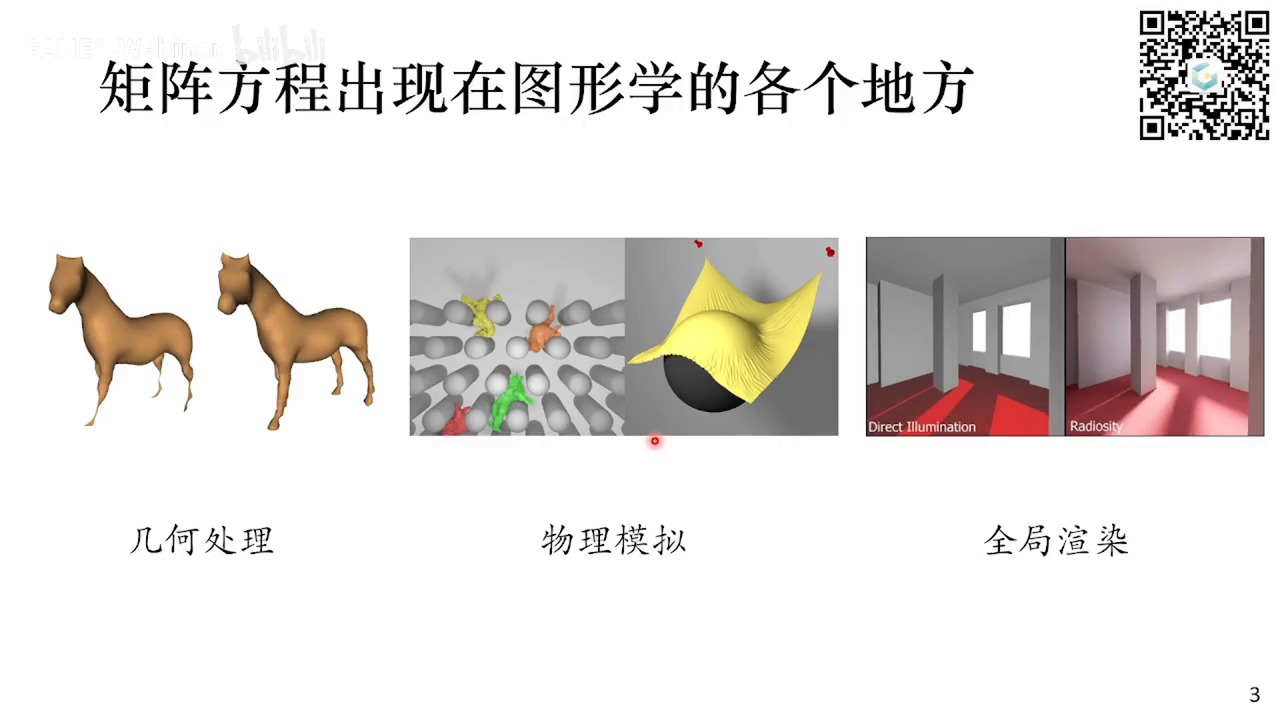
\includegraphics[width=0.92\textwidth]{figures/fig_01_applications.jpg}
\caption{矩阵方程出现在图形学的各个地方：几何处理、物理模拟与全局渲染\vtag}
\end{figure}
\srcnote{00:01:15--00:01:30}
\end{minipage}


本讲分为三部分：直接求解（高斯消元、LU 分解、主元选择、科列斯基分解）；第一类迭代方法，不动点迭代（雅可比迭代、收敛准则、松弛、高斯—赛德尔迭代）；第二类迭代方法，子空间迭代（Krylov 子空间、共轭梯度下降、预处理以及其他 Krylov 求解器）。

\begin{importantbox}{本讲的主线}
直接法把矩阵分解成三角矩阵，复杂度 $O(n^3)$，适合小矩阵；迭代法从初始猜解出发反复改进，适合图形学里常见的大规模稀疏矩阵。不动点迭代的收敛取决于迭代矩阵的谱半径，子空间迭代（以共轭梯度为代表）的收敛取决于条件数。预处理的本质，是用一个容易求逆的近似 $\mathrm{M}\approx\mathrm{A}$ 或 $\mathrm{M}\approx\mathrm{A}^{-1}$ 来改善这两个量。
\end{importantbox}

\section{直接求解：高斯消元}

\subsection{一个三乘三的例子}

\noindent\begin{minipage}{\textwidth}
\begin{figure}[H]
\centering
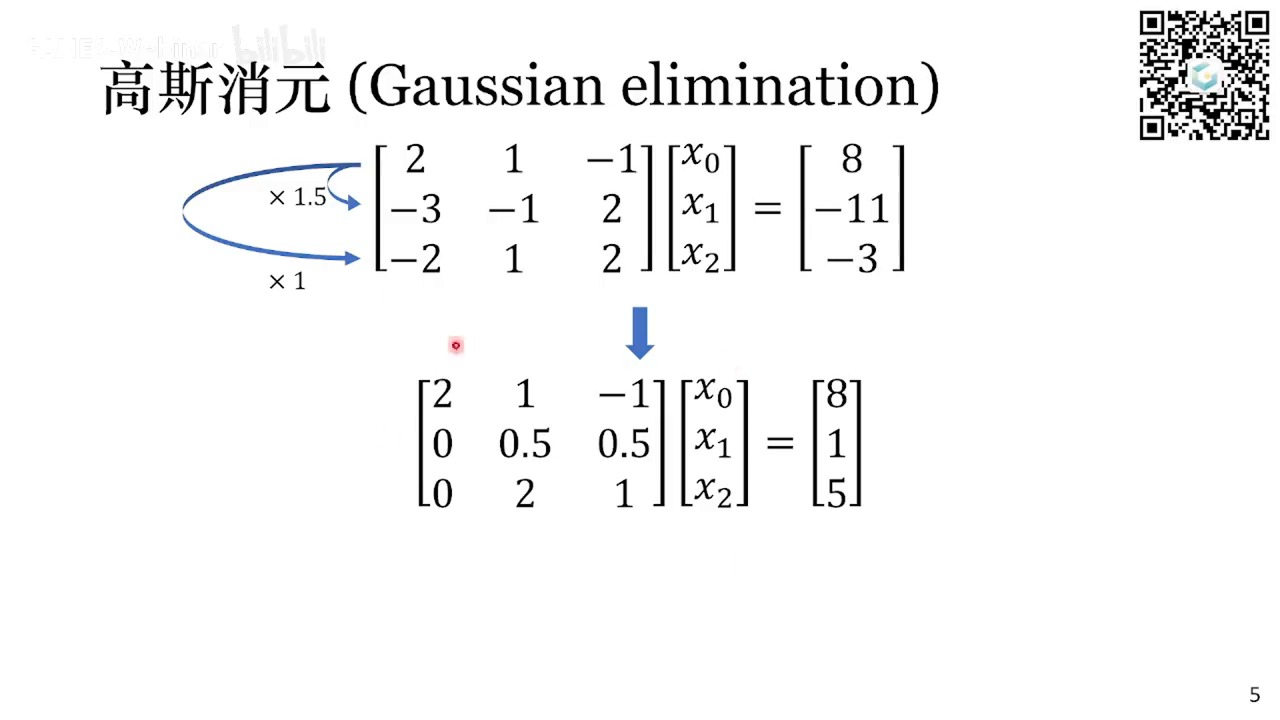
\includegraphics[width=0.92\textwidth]{figures/fig_02_gauss1.jpg}
\caption{高斯消元：用第一行消去下面两行的第一个元素\vtag}
\end{figure}
\srcnote{00:02:15--00:02:30}
\end{minipage}


大家在学习线性代数时应该学过用高斯消元法解方程。以这个三乘三的矩阵为例：
\begin{equation}
\begin{pmatrix}2&1&-1\\-3&-1&2\\-2&1&2\end{pmatrix}\begin{pmatrix}x_0\\x_1\\x_2\end{pmatrix}=\begin{pmatrix}8\\-11\\-3\end{pmatrix}.
\end{equation}
第一步，把第一行乘以 $1.5$ 加到第二行，第二行第一个元素 $-3+2\times 1.5$ 就变成零，右端 $-11+8\times 1.5=1$；再把第一行乘以 $1$ 加到最后一行，把 $-2$ 消掉。得到
\begin{equation}
\begin{pmatrix}2&1&-1\\0&0.5&0.5\\0&2&1\end{pmatrix}\begin{pmatrix}x_0\\x_1\\x_2\end{pmatrix}=\begin{pmatrix}8\\1\\5\end{pmatrix}.
\end{equation}

\noindent\begin{minipage}{\textwidth}
\begin{figure}[H]
\centering
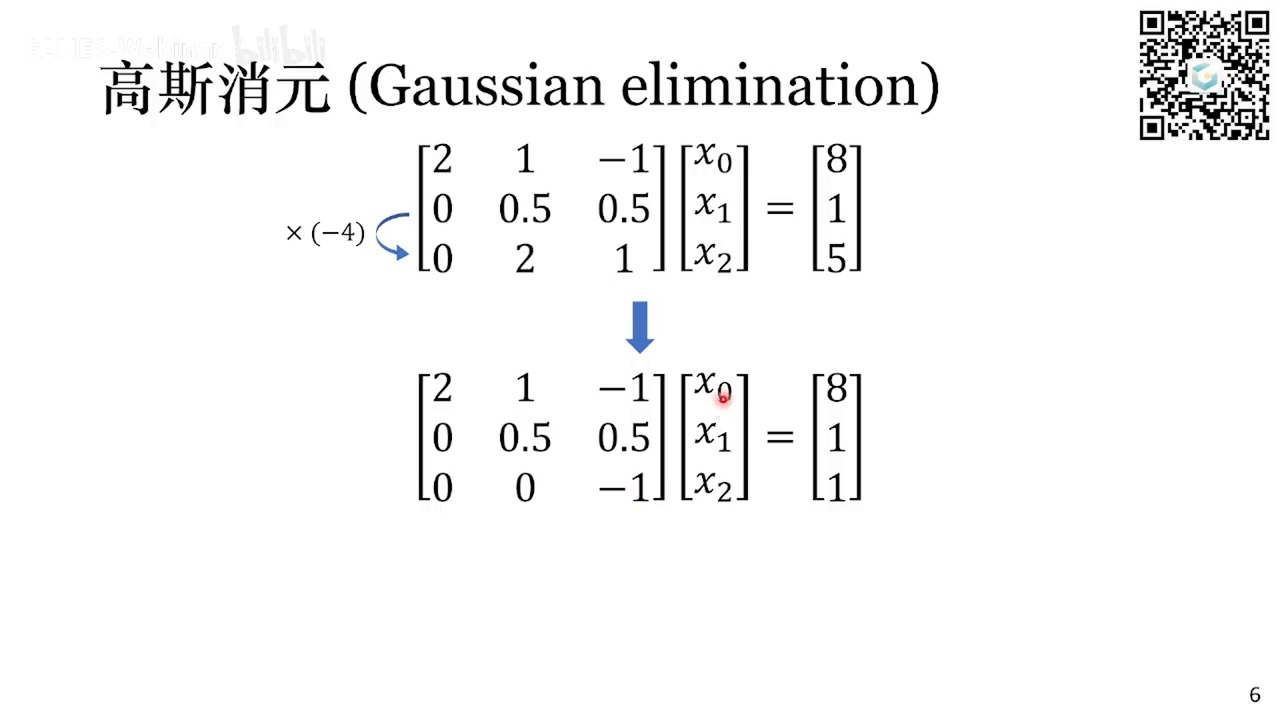
\includegraphics[width=0.92\textwidth]{figures/fig_03_gauss2.jpg}
\caption{高斯消元：用第二行消去第三行，得到上三角矩阵\vtag}
\end{figure}
\srcnote{00:03:00--00:03:15}
\end{minipage}


第二步，把第二行乘以 $-4$ 加到第三行，消去第三行的第二个元素，得到上三角矩阵
\begin{equation}
\begin{pmatrix}2&1&-1\\0&0.5&0.5\\0&0&-1\end{pmatrix}\begin{pmatrix}x_0\\x_1\\x_2\end{pmatrix}=\begin{pmatrix}8\\1\\1\end{pmatrix}.
\end{equation}

\noindent\begin{minipage}{\textwidth}
\begin{figure}[H]
\centering
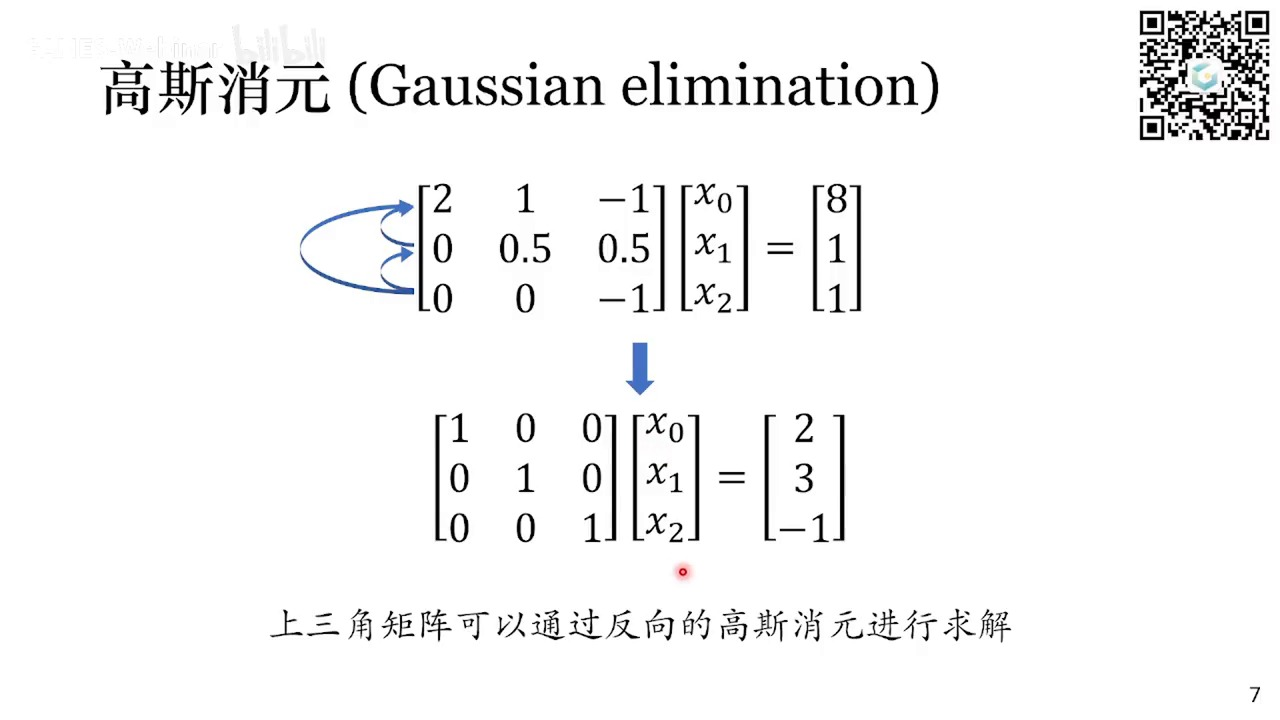
\includegraphics[width=0.92\textwidth]{figures/fig_04_gauss_back.jpg}
\caption{上三角矩阵可以通过反向的高斯消元进行求解\vtag}
\end{figure}
\srcnote{00:03:30--00:03:45}
\end{minipage}


上三角矩阵可以通过反向的高斯消元求解：先解最后一行得 $x_2$，再解倒数第二行得 $x_1$，再解第一行得 $x_0$，把所有的值求出来，结果为 $x=(2,3,-1)^{\mathsf T}$。

\subsection{行变换与 LU 分解}

\noindent\begin{minipage}{\textwidth}
\begin{figure}[H]
\centering
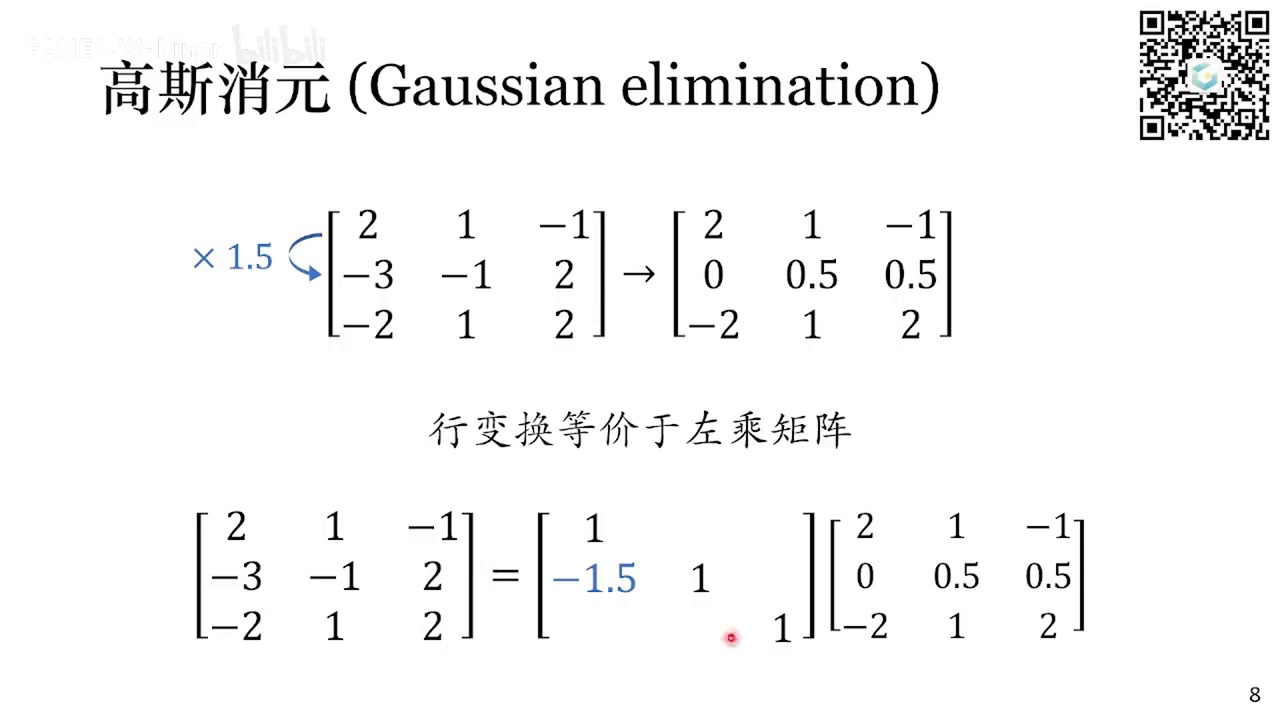
\includegraphics[width=0.92\textwidth]{figures/fig_05_row_op.jpg}
\caption{行变换等价于左乘矩阵\vtag}
\end{figure}
\srcnote{00:05:15--00:05:30}
\end{minipage}


每一次行变换都等价于左乘一个矩阵。比如把第一行乘以 $1.5$ 加到第二行、乘以 $1$ 加到第三行，等价于左乘
\begin{equation}
\begin{pmatrix}1&&\\1.5&1&\\1&&1\end{pmatrix}\begin{pmatrix}2&1&-1\\-3&-1&2\\-2&1&2\end{pmatrix}=\begin{pmatrix}2&1&-1\\0&0.5&0.5\\0&2&1\end{pmatrix}.
\end{equation}
这个矩阵的逆也很好求：把 $1.5$ 和 $1$ 取相反数即可，相当于再把加上去的减回来，恢复第二行原来的值。

\noindent\begin{minipage}{\textwidth}
\begin{figure}[H]
\centering
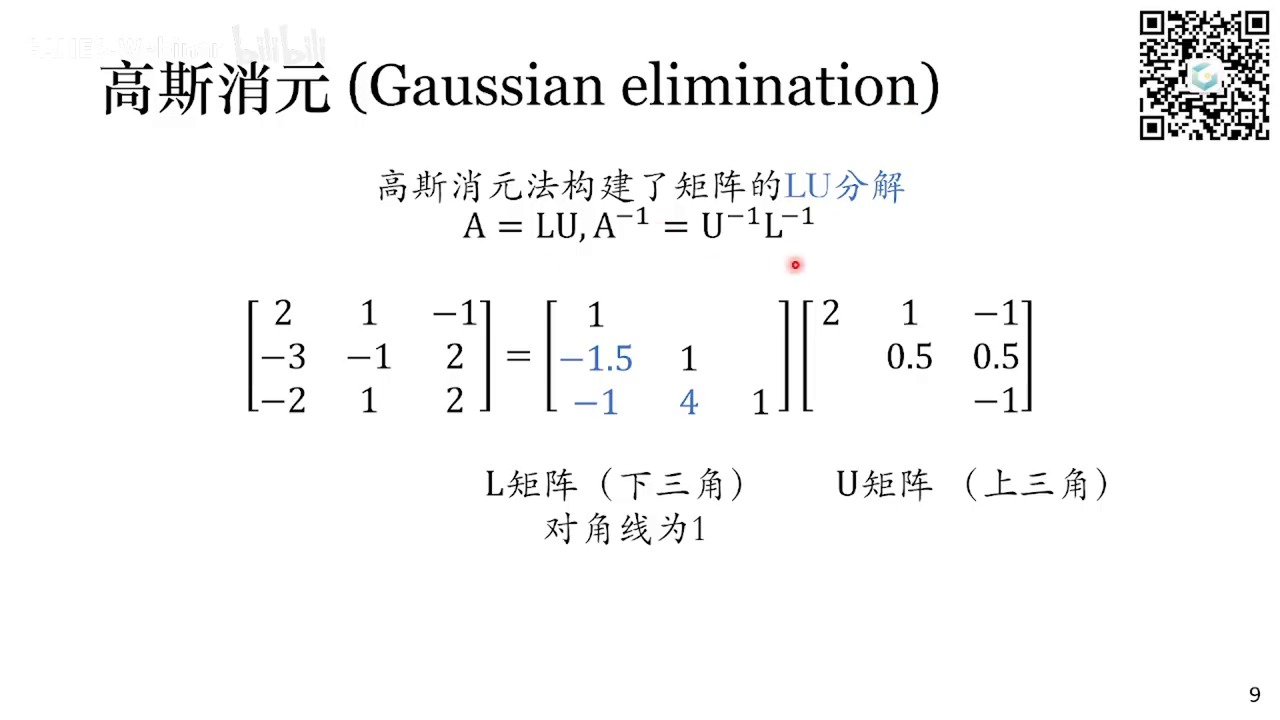
\includegraphics[width=0.92\textwidth]{figures/fig_06_lu.jpg}
\caption{高斯消元法构建了矩阵的 LU 分解\vtag}
\end{figure}
\srcnote{00:08:00--00:08:15}
\end{minipage}


把所有行变换的逆乘起来，就得到一个下三角矩阵。讲者让大家倒回去看用了哪些系数：$1.5$、$1$，还有 $-4$，它们取相反数后正好出现在下三角矩阵中。于是高斯消元法构建了矩阵的 LU 分解：
\begin{equation}
\begin{pmatrix}2&1&-1\\-3&-1&2\\-2&1&2\end{pmatrix}=
\begin{pmatrix}1&&\\-1.5&1&\\-1&4&1\end{pmatrix}
\begin{pmatrix}2&1&-1\\&0.5&0.5\\&&-1\end{pmatrix},
\end{equation}
$\mathrm{A}=\mathrm{LU}$，$\mathrm{A}^{-1}=\mathrm{U}^{-1}\mathrm{L}^{-1}$。L 矩阵是下三角的，对角线为一；U 矩阵是上三角的。有了 LU 分解，解 $\mathrm{A}x=b$ 时先把 $\mathrm{U}x$ 看成整体去解下三角方程 $\mathrm{L}y=b$，再解上三角方程 $\mathrm{U}x=y$，两步都很容易。

\begin{knowledgebox}{分解一次，求解多次}
讲义作者补充：LU 分解的代价是 $O(n^3)$，但之后每解一个新的右端 $b$ 只需两次三角回代，代价是 $O(n^2)$。在物理模拟中，如果系统矩阵不随时间变化（例如固定刚度的隐式弹簧），就可以预先分解一次，每一帧只做回代，这比每帧重新求解快得多。
\end{knowledgebox}

\subsection{LU 分解算法}

\noindent\begin{minipage}{\textwidth}
\begin{figure}[H]
\centering
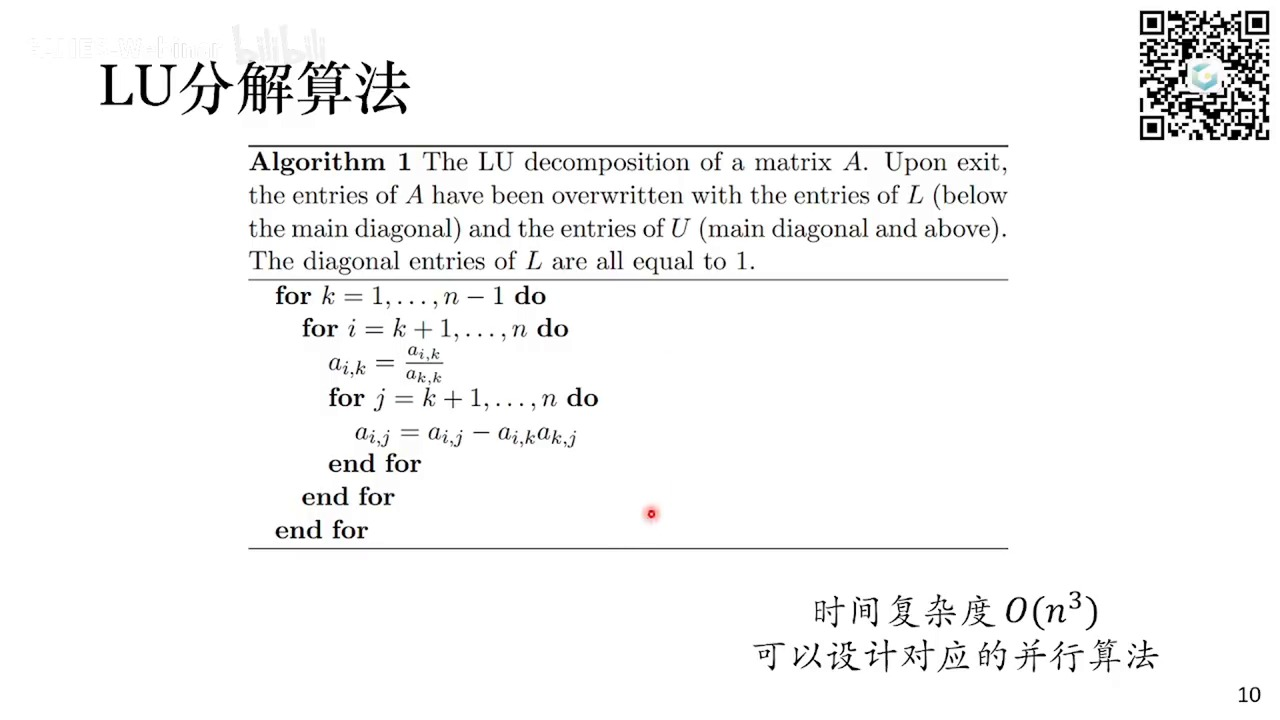
\includegraphics[width=0.92\textwidth]{figures/fig_07_lu_algo.jpg}
\caption{LU 分解算法\vtag}
\end{figure}
\srcnote{00:09:30--00:09:45}
\end{minipage}


课件给出了 LU 分解的基本算法，流程就是刚才手算的过程。它的复杂度很容易看出：有三重 for 循环，时间复杂度为 $O(n^3)$，也可以设计对应的并行算法。

\subsection{主元选择}

\noindent\begin{minipage}{\textwidth}
\begin{figure}[H]
\centering
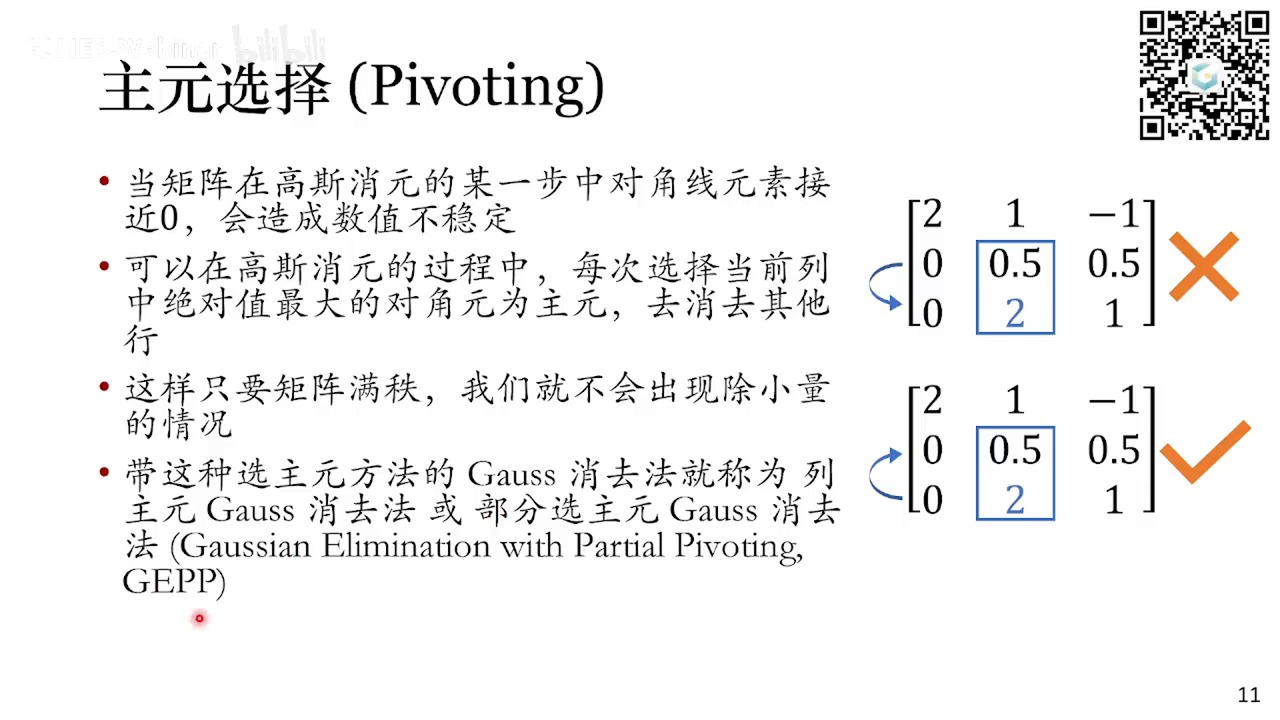
\includegraphics[width=0.92\textwidth]{figures/fig_08_pivoting.jpg}
\caption{主元选择：避免在对角线元素接近零时除以小量\vtag}
\end{figure}
\srcnote{00:11:15--00:11:30}
\end{minipage}


假如刚才例子中第二行第二列的位置不是 $0.5$ 而是 $0$，这是有可能发生的：第一行消第二行时，刚好不光把第一个元素消掉了，还把第二个元素也消成零。这时就无法用它去消下面的行。更一般地，当矩阵在高斯消元的某一步中对角线元素接近零时，就会造成数值不稳定。

解决办法是：在高斯消元的过程中，每次选择当前列中绝对值最大的元素作为主元，交换到对角线上，再去消其他行。这样只要矩阵满秩，就不会出现除以小量的情况。带这种选主元方法的高斯消去法称为列主元高斯消去法或部分选主元高斯消去法（Gaussian elimination with partial pivoting，GEPP）。在上例中，用第三行的 $2$ 而不是第二行的 $0.5$ 作为第二列的主元更稳定。

\begin{warningbox}{不选主元的代价}
讲义作者用一个小例子说明：$\begin{pmatrix}\varepsilon&1\\1&1\end{pmatrix}$ 当 $\varepsilon$ 很小时，若直接用 $\varepsilon$ 作主元，消元会产生 $1-1/\varepsilon$ 这样的巨大数，舍入误差被放大，解可能完全错误；交换两行后再消元则没有问题。矩阵本身条件很好，坏的只是消元顺序。
\end{warningbox}

\section{科列斯基分解}

\noindent\begin{minipage}{\textwidth}
\begin{figure}[H]
\centering
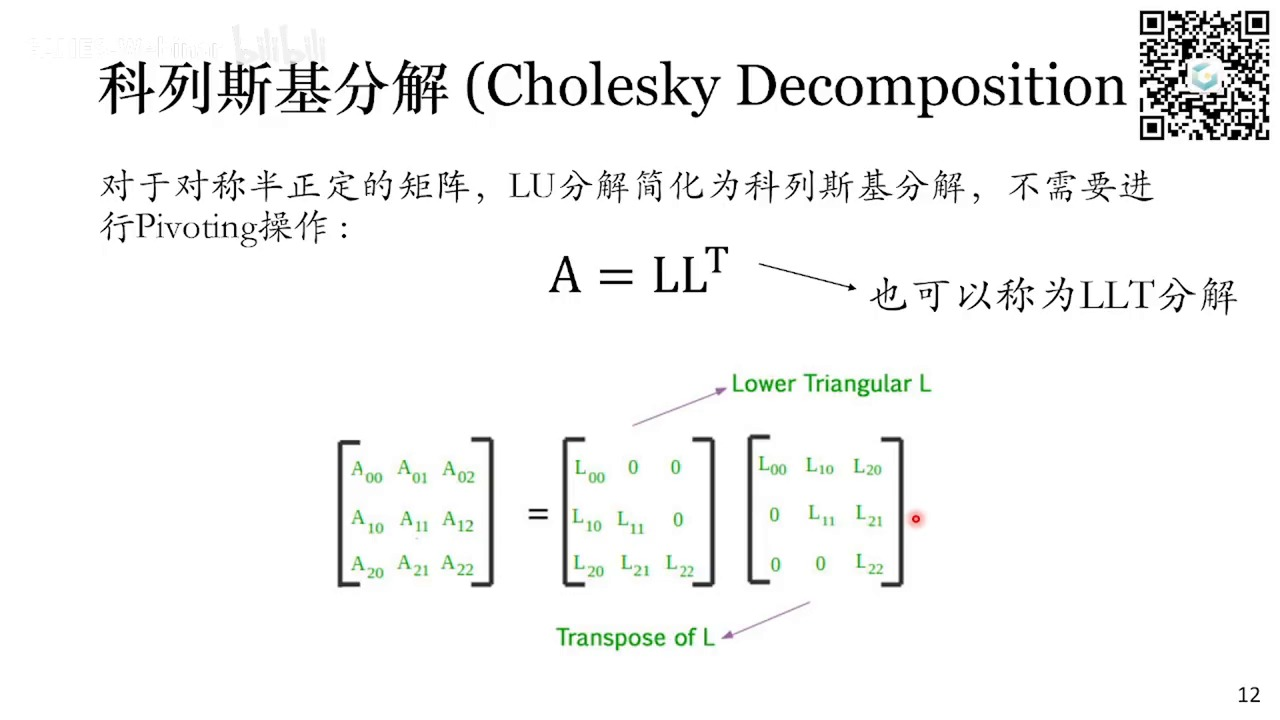
\includegraphics[width=0.92\textwidth]{figures/fig_09_cholesky.jpg}
\caption{科列斯基分解：对称正定矩阵的 $\mathrm{LL}^{\mathsf T}$ 分解\vtag}
\end{figure}
\srcnote{00:12:15--00:12:30}
\end{minipage}


对于对称半正定的矩阵，LU 分解可以简化为科列斯基分解，并且不需要进行主元选择操作：
\begin{equation}
\mathrm{A}=\mathrm{LL}^{\mathsf T},
\end{equation}
也可以称为 $\mathrm{LL}^{\mathsf T}$ 分解。L 是下三角矩阵，$\mathrm{L}^{\mathsf T}$ 是上三角矩阵，所以依然是把 A 分解成下三角矩阵乘以上三角矩阵，只不过两者互为转置。

\noindent\begin{minipage}{\textwidth}
\begin{figure}[H]
\centering
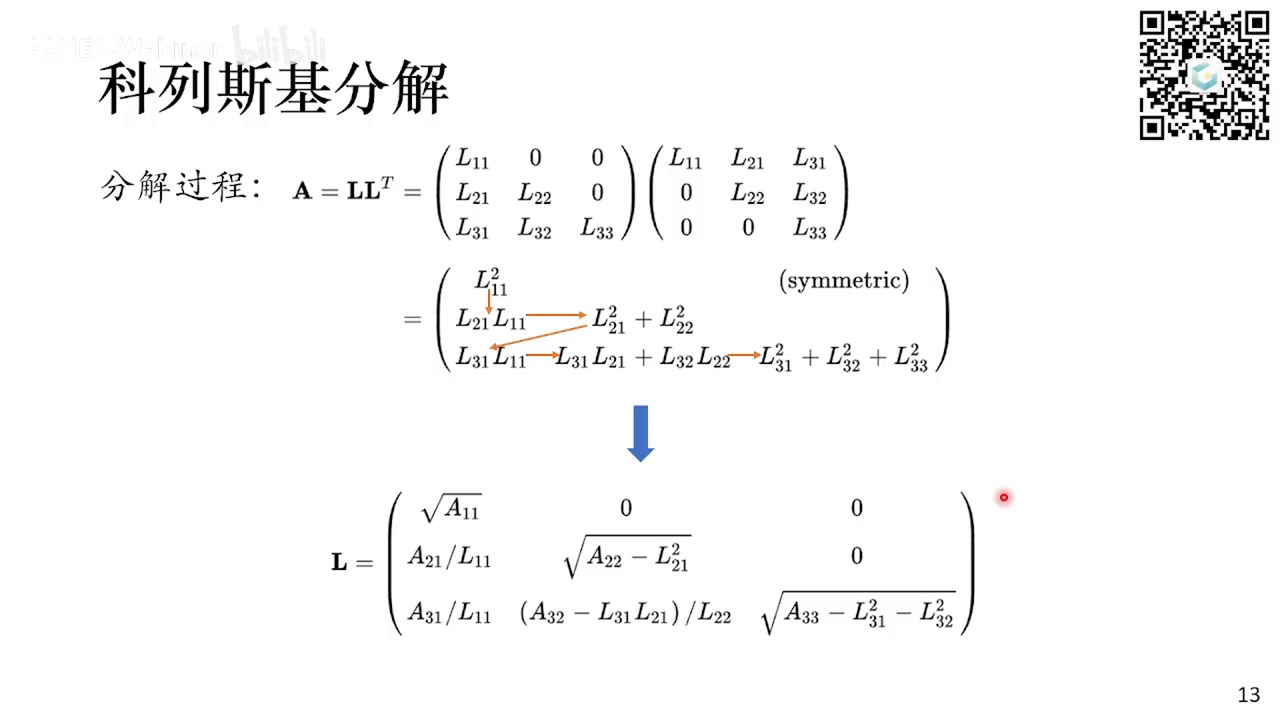
\includegraphics[width=0.92\textwidth]{figures/fig_10_cholesky_steps.jpg}
\caption{科列斯基分解的过程\vtag}
\end{figure}
\srcnote{00:13:45--00:14:00}
\end{minipage}


分解过程：把 $\mathrm{A}$ 与 $\mathrm{LL}^{\mathsf T}$ 逐元素比较，以三阶为例，
\begin{equation}
\mathrm{L}=\begin{pmatrix}\sqrt{A_{11}}&0&0\\ A_{21}/L_{11}&\sqrt{A_{22}-L_{21}^2}&0\\ A_{31}/L_{11}&(A_{32}-L_{31}L_{21})/L_{22}&\sqrt{A_{33}-L_{31}^2-L_{32}^2}\end{pmatrix}.
\end{equation}
可以按列从左到右依次算出 L 的每一个元素。

\begin{warningbox}{“半正定”还是“正定”}
课件写的是对称半正定矩阵。讲义作者提醒：标准的科列斯基分解要求矩阵对称正定，因为对角线上要开平方并作为除数；半正定矩阵可能在某一步出现 $L_{ii}=0$，后面的除法就无法进行。实际使用时（例如 Eigen 的 \texttt{LLT}），通常要求严格正定，半正定的情形可改用带主元的 $\mathrm{LDL}^{\mathsf T}$ 分解。
\end{warningbox}

\noindent\begin{minipage}{\textwidth}
\begin{figure}[H]
\centering
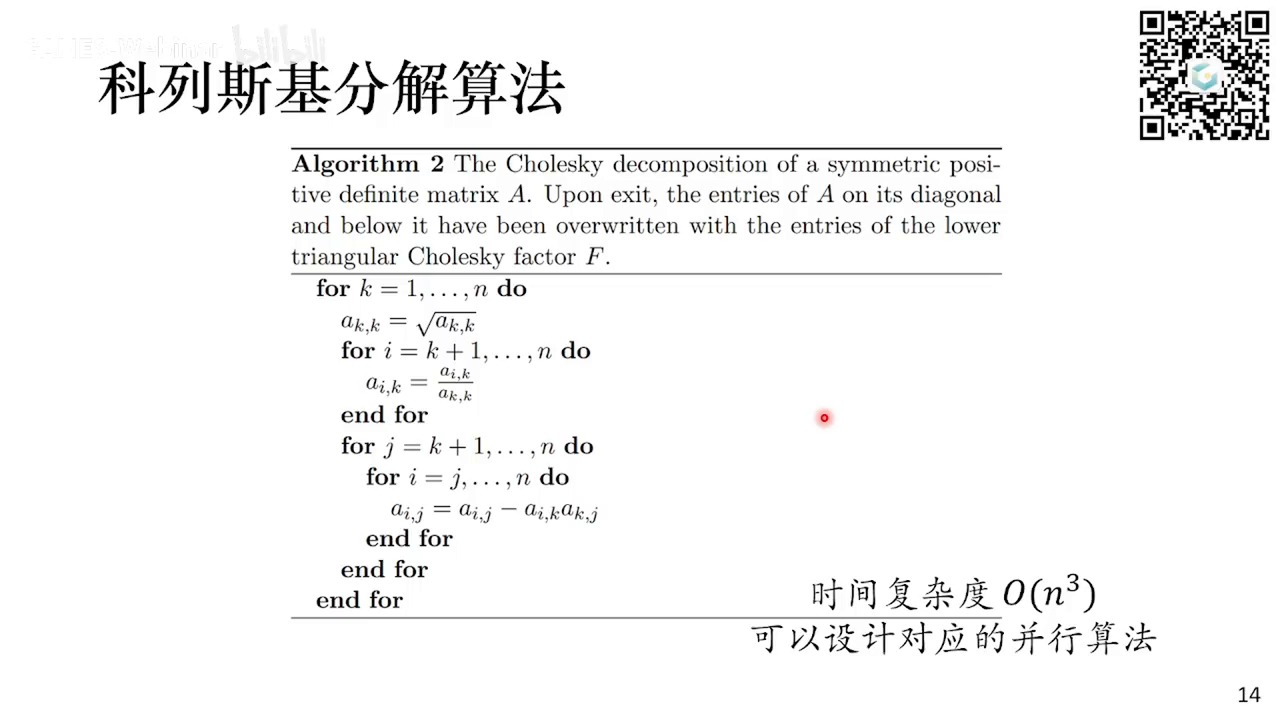
\includegraphics[width=0.92\textwidth]{figures/fig_11_cholesky_algo.jpg}
\caption{科列斯基分解算法\vtag}
\end{figure}
\srcnote{00:14:15--00:14:30}
\end{minipage}


科列斯基分解算法和刚才的 LU 分解比较像，同样有三重 for 循环，时间复杂度也是 $O(n^3)$，也可以设计对应的并行算法。它只适用于对称（正定）的情况，但相应地，速度会比 LU 分解更快一点，大约只需一半的运算量，也不会有除零的问题。

\subsection{直接求解法的局限}

\noindent\begin{minipage}{\textwidth}
\begin{figure}[H]
\centering
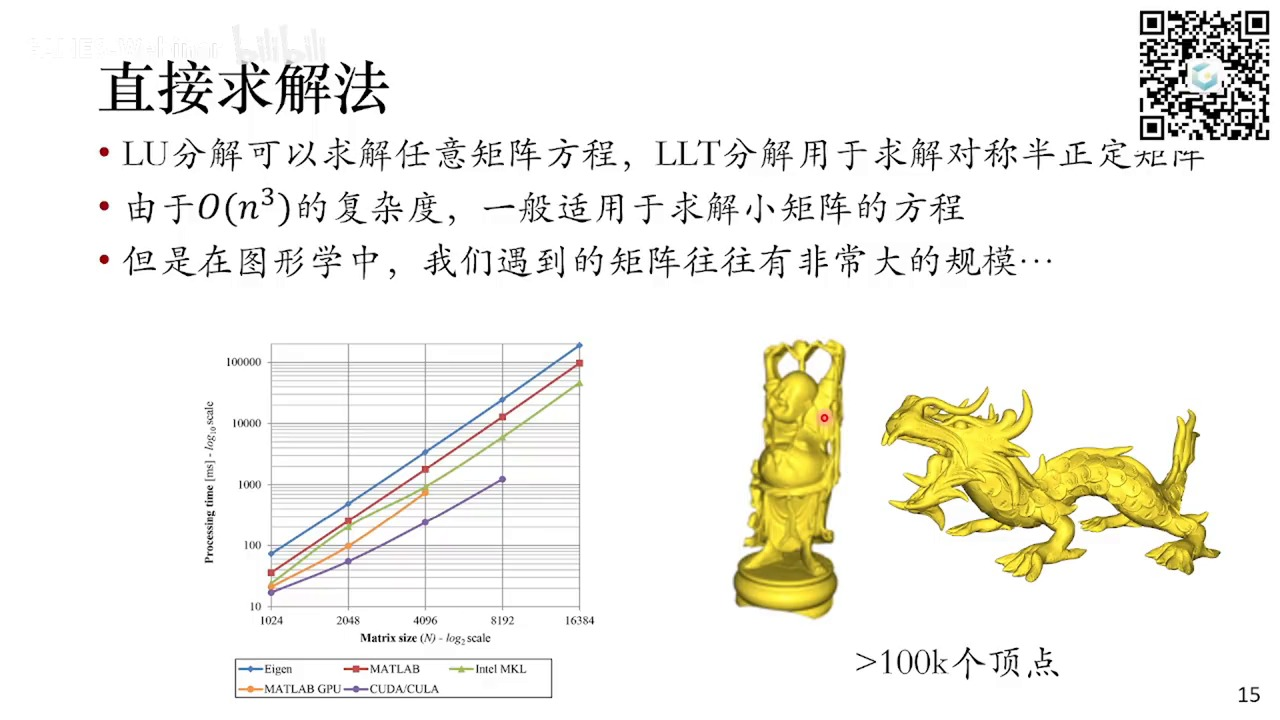
\includegraphics[width=0.92\textwidth]{figures/fig_12_direct_limit.jpg}
\caption{直接求解法的局限：图形学中的矩阵规模往往非常大\vtag}
\end{figure}
\srcnote{00:16:15--00:16:30}
\end{minipage}


LU 分解可以求解任意（可逆）矩阵方程，$\mathrm{LL}^{\mathsf T}$ 分解用于求解对称正定矩阵。由于 $O(n^3)$ 的复杂度，它们一般适用于求解小矩阵的方程。但在图形学中，矩阵的规模往往非常大：图中展示的网格轻轻松松就有十万个以上的顶点。讲者说，这样的方程再用 LU 分解会非常非常慢，可能需要几十分钟甚至几个小时，这显然不可接受。所以对大规模矩阵方程，一般使用迭代求解的方法。

\section{迭代求解}

\subsection{迭代方法的流程与优点}

\noindent\begin{minipage}{\textwidth}
\begin{figure}[H]
\centering
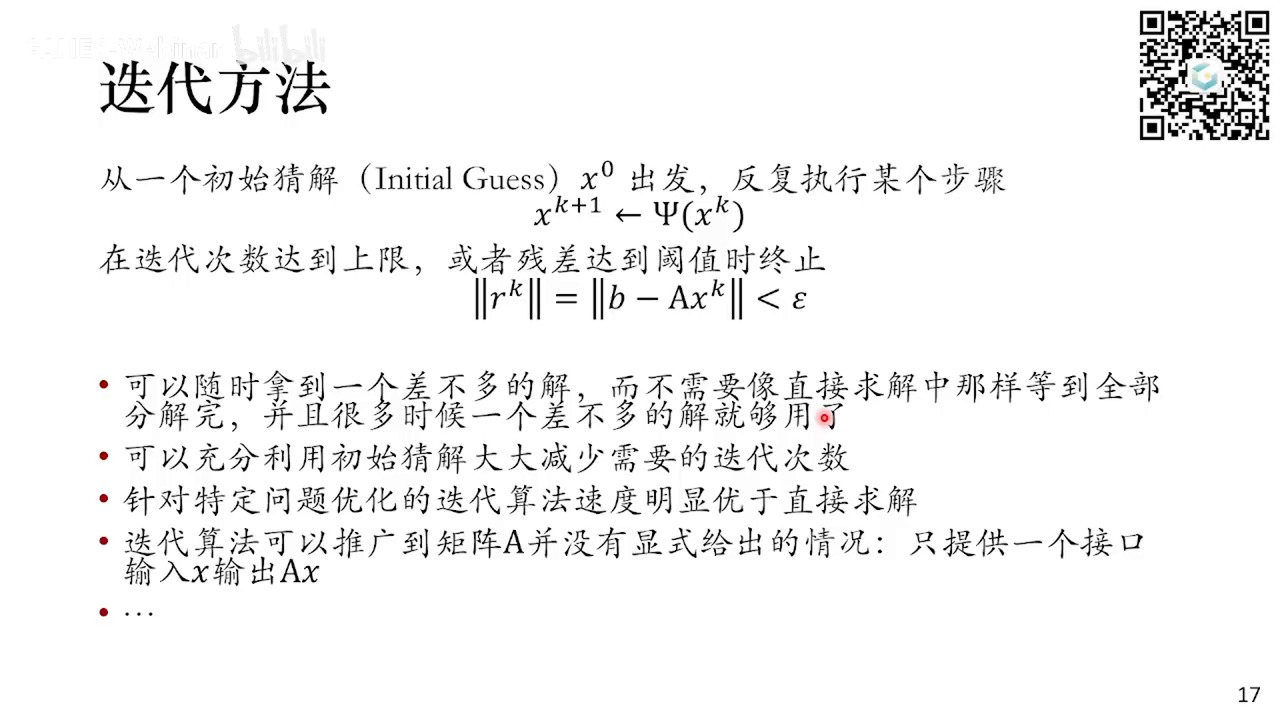
\includegraphics[width=0.92\textwidth]{figures/fig_13_iterative.jpg}
\caption{迭代方法：从初始猜解出发反复执行某个步骤\vtag}
\end{figure}
\srcnote{00:20:00--00:20:15}
\end{minipage}


迭代方法从一个初始猜解（initial guess）$x^0$ 出发，反复执行某个步骤
\begin{equation}
x^{k+1}\leftarrow\Psi(x^k),
\end{equation}
在迭代次数达到上限，或者残差达到阈值时终止：$\|r^k\|=\|b-\mathrm{A}x^k\|<\varepsilon$。讲者说，如果没有任何信息，可以直接把 $x^0$ 置成零；如果大概知道解可能是多少，就把它作为初始值。而且很多情况下，残差并不需要降到 $10^{-3}$、$10^{-4}$ 那么小。

迭代方法相对直接求解有这些好处：
\begin{itemize}
\item 可以随时拿到一个差不多的解，而不需要像直接求解那样等到全部分解完，并且很多时候一个差不多的解就够用了；
\item 可以充分利用初始猜解，大大减少需要的迭代次数；
\item 针对特定问题（比如稀疏、对称的矩阵）优化的迭代算法，速度明显优于直接求解；
\item 迭代算法可以推广到矩阵 A 并没有显式给出的情况：只要提供一个接口，输入 $x$、输出 $\mathrm{A}x$ 即可。
\end{itemize}

\noindent\begin{minipage}{\textwidth}
\begin{figure}[H]
\centering
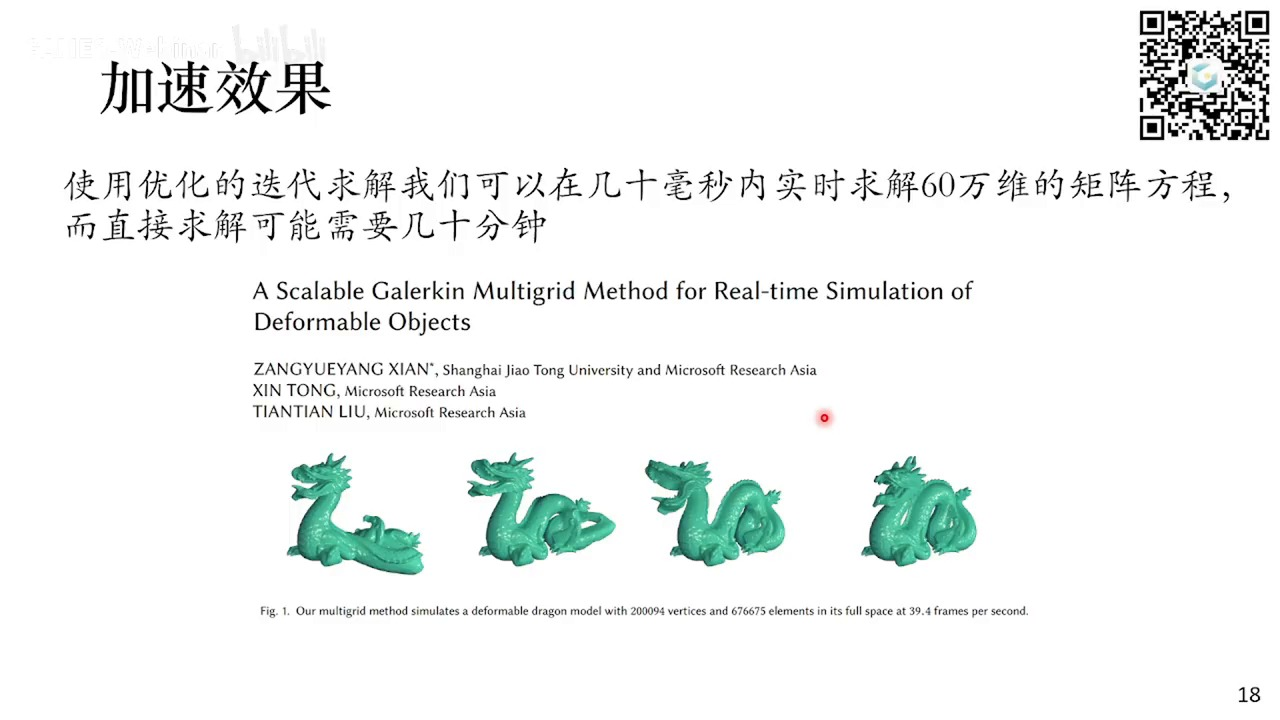
\includegraphics[width=0.92\textwidth]{figures/fig_14_speedup.jpg}
\caption{加速效果：优化的迭代求解可以在几十毫秒内求解六十万维的矩阵方程\vtag}
\end{figure}
\srcnote{00:20:45--00:21:00}
\end{minipage}


课件展示了一个例子：使用优化的迭代求解，可以在几十毫秒内实时求解 $60$ 万维的矩阵方程，而直接求解可能需要几十分钟。

\begin{importantbox}{“矩阵无需显式给出”的意义}
讲义作者补充：迭代法只需要矩阵—向量乘积。在物理模拟中，系统矩阵往往是许多小块（每个单元、每根弹簧）贡献之和，可以在不组装大矩阵的情况下直接计算 $\mathrm{A}x$，这叫无矩阵（matrix-free）方法，在 GPU 上尤其高效。这是直接法做不到的。
\end{importantbox}

\section{第一类：不动点迭代}

\subsection{一个简单的例子}

\noindent\begin{minipage}{\textwidth}
\begin{figure}[H]
\centering
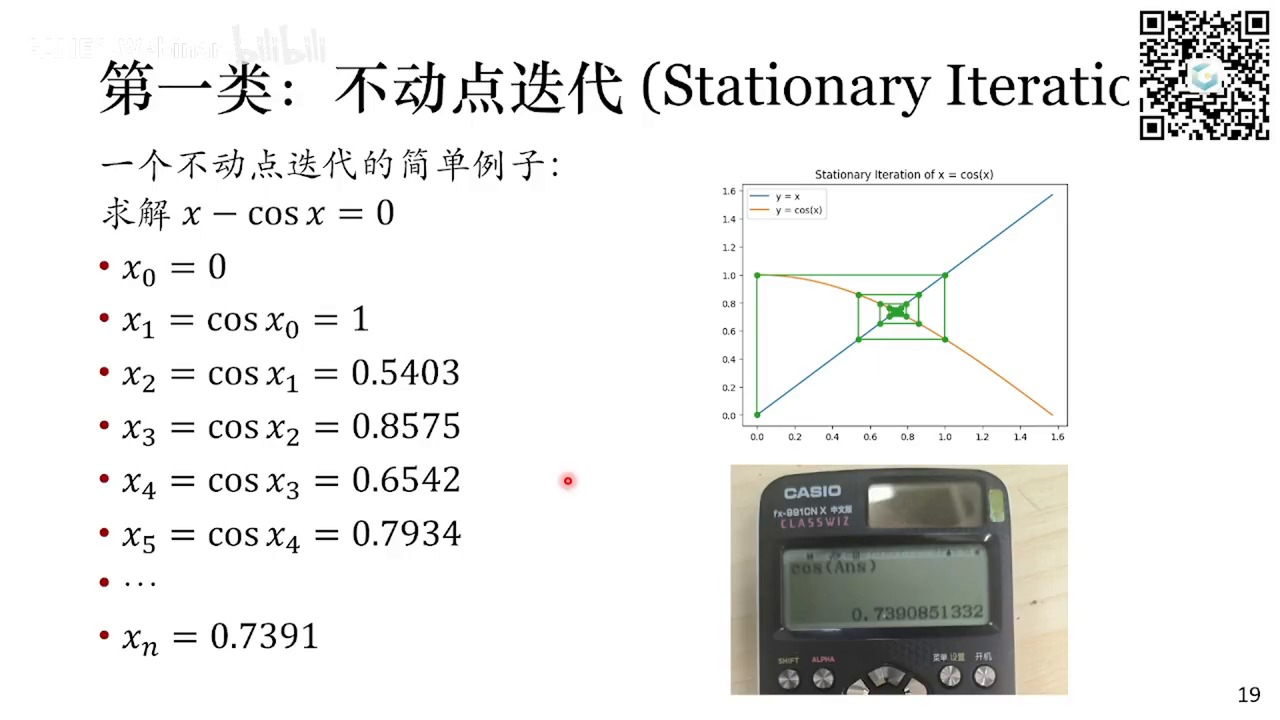
\includegraphics[width=0.92\textwidth]{figures/fig_15_fixed_point.jpg}
\caption{不动点迭代的简单例子：求解 $x-\cos x=0$\vtag}
\end{figure}
\srcnote{00:22:45--00:23:00}
\end{minipage}


讲者举了一个非常简单的例子：如果玩过卡西欧计算器，可以试试这样操作。随便给一个初始值，比如 $x_0=0$，不断地执行 $\cos(\mathrm{Ans})$：
\begin{equation}
x_1=\cos x_0=1,\quad x_2=\cos x_1=0.5403,\quad x_3=0.8575,\quad x_4=0.6542,\quad x_5=0.7934,\quad\dots
\end{equation}
一直按等号，最终会得到 $x_n=0.7391$，这就是 $x-\cos x=0$ 的解。图中蓝线是 $y=x$，橙线是 $y=\cos x$，迭代在两条线之间来回跳，最后收敛到交点。

\subsection{矩阵方程的不动点迭代}

\noindent\begin{minipage}{\textwidth}
\begin{figure}[H]
\centering
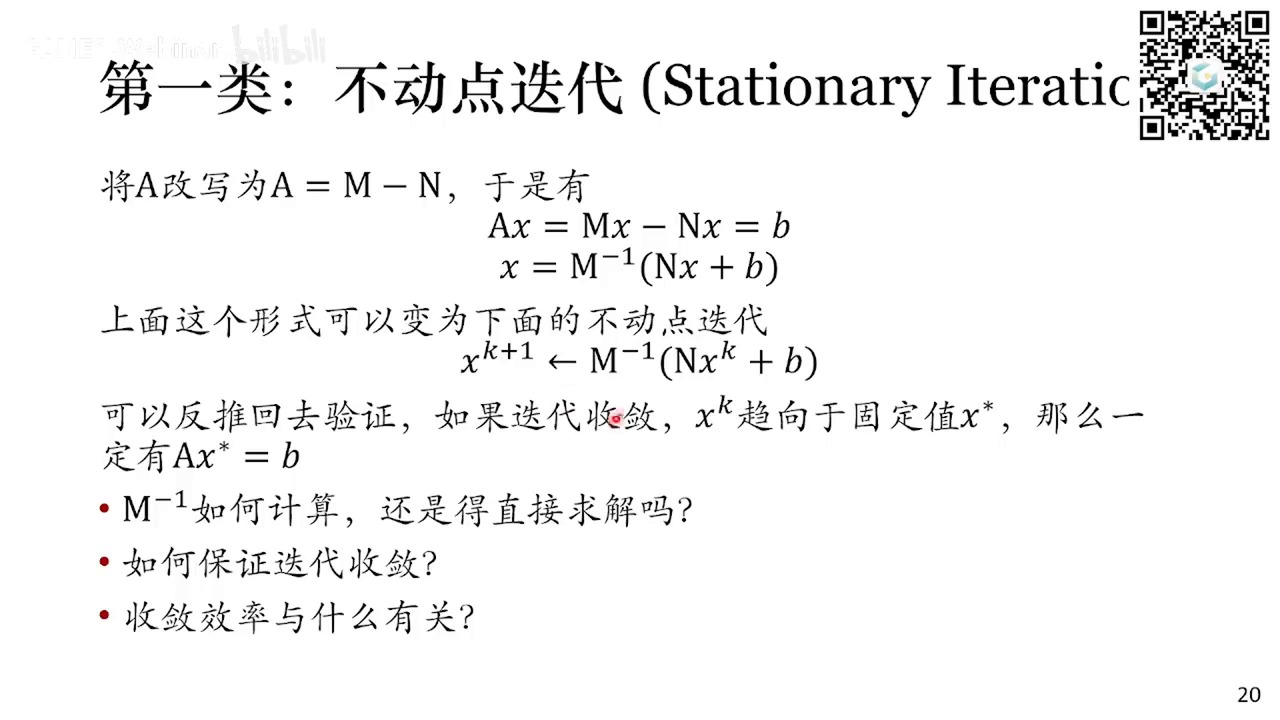
\includegraphics[width=0.92\textwidth]{figures/fig_16_stationary.jpg}
\caption{将 A 拆成 M 与 N 之差，构造不动点迭代\vtag}
\end{figure}
\srcnote{00:25:15--00:25:30}
\end{minipage}


换到矩阵方程，把 A 改写为两个矩阵之差 $\mathrm{A}=\mathrm{M}-\mathrm{N}$，于是有
\begin{equation}
\mathrm{A}x=\mathrm{M}x-\mathrm{N}x=b\quad\Longrightarrow\quad x=\mathrm{M}^{-1}(\mathrm{N}x+b).
\end{equation}
这个形式可以变为不动点迭代：把 $x^k$ 代入右边，输出的结果作为 $x^{k+1}$，下一步再代入，如此往复：
\begin{equation}
x^{k+1}\leftarrow\mathrm{M}^{-1}(\mathrm{N}x^k+b).
\end{equation}
可以反推回去验证：如果迭代收敛，$x^k$ 趋向于固定值 $x^*$，那么一定有 $\mathrm{A}x^*=b$。

讲者提出三个问题：$\mathrm{M}^{-1}$ 如何计算，还是得直接求解吗？如何保证迭代收敛？收敛效率与什么有关？

\subsection{雅可比迭代}

\noindent\begin{minipage}{\textwidth}
\begin{figure}[H]
\centering
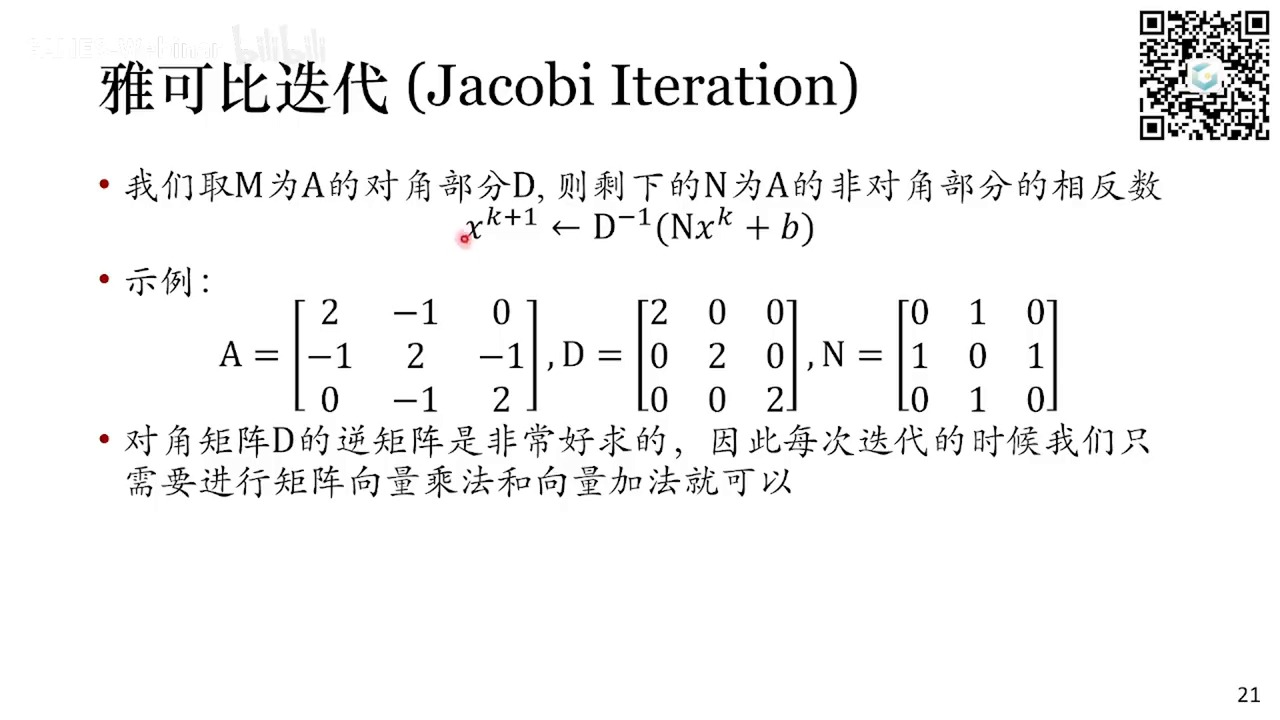
\includegraphics[width=0.92\textwidth]{figures/fig_17_jacobi.jpg}
\caption{雅可比迭代：取 M 为 A 的对角部分\vtag}
\end{figure}
\srcnote{00:26:15--00:26:30}
\end{minipage}


雅可比迭代取 M 为 A 的对角部分 D，则剩下的 N 为 A 的非对角部分的相反数：
\begin{equation}
x^{k+1}\leftarrow\mathrm{D}^{-1}(\mathrm{N}x^k+b).
\end{equation}
示例：
\begin{equation}
\mathrm{A}=\begin{pmatrix}2&-1&0\\-1&2&-1\\0&-1&2\end{pmatrix},\quad
\mathrm{D}=\begin{pmatrix}2&0&0\\0&2&0\\0&0&2\end{pmatrix},\quad
\mathrm{N}=\begin{pmatrix}0&1&0\\1&0&1\\0&1&0\end{pmatrix}.
\end{equation}
对角矩阵 D 的逆矩阵非常好求，所以每次迭代只需要进行矩阵向量乘法和向量加法。

\noindent\begin{minipage}{\textwidth}
\begin{figure}[H]
\centering
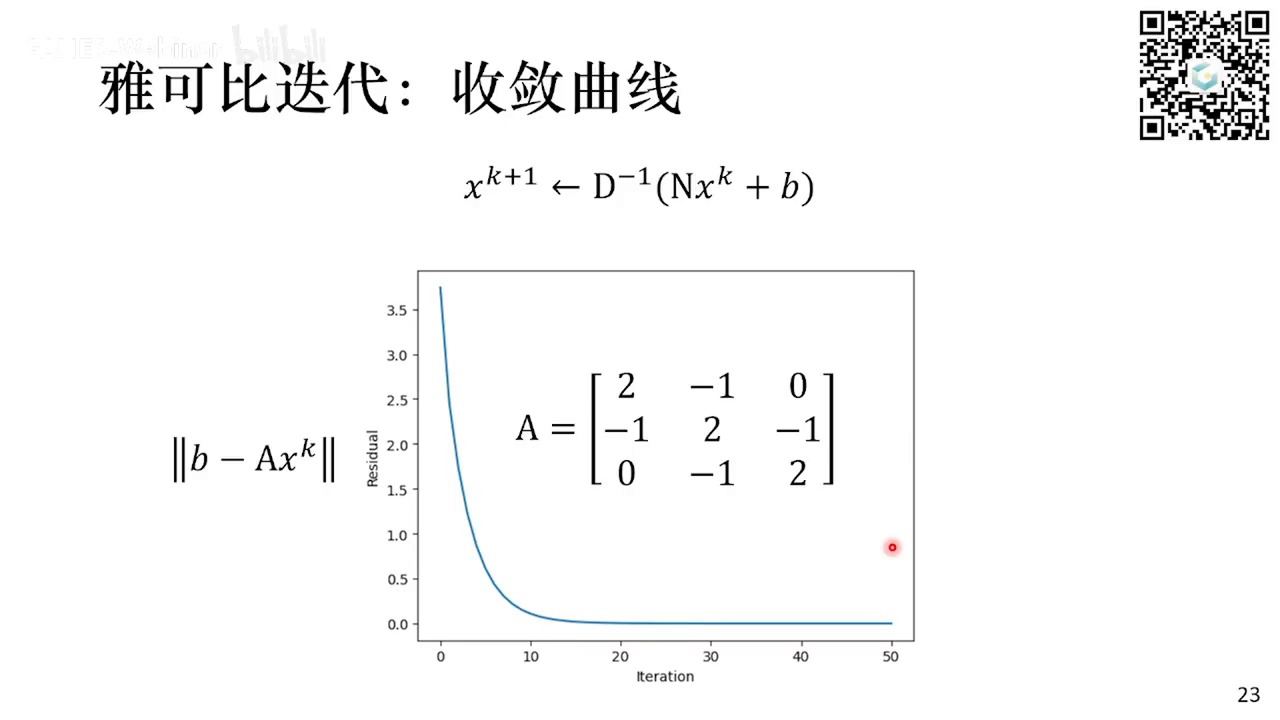
\includegraphics[width=0.92\textwidth]{figures/fig_18_jacobi_curve.jpg}
\caption{雅可比迭代的收敛曲线：残差 $\|b-\mathrm{A}x^k\|$ 随迭代下降\vtag}
\end{figure}
\srcnote{00:27:30--00:27:45}
\end{minipage}


对上面这个矩阵，残差 $\|b-\mathrm{A}x^k\|$ 随迭代次数稳定下降，雅可比迭代收敛。

\noindent\begin{minipage}{\textwidth}
\begin{figure}[H]
\centering
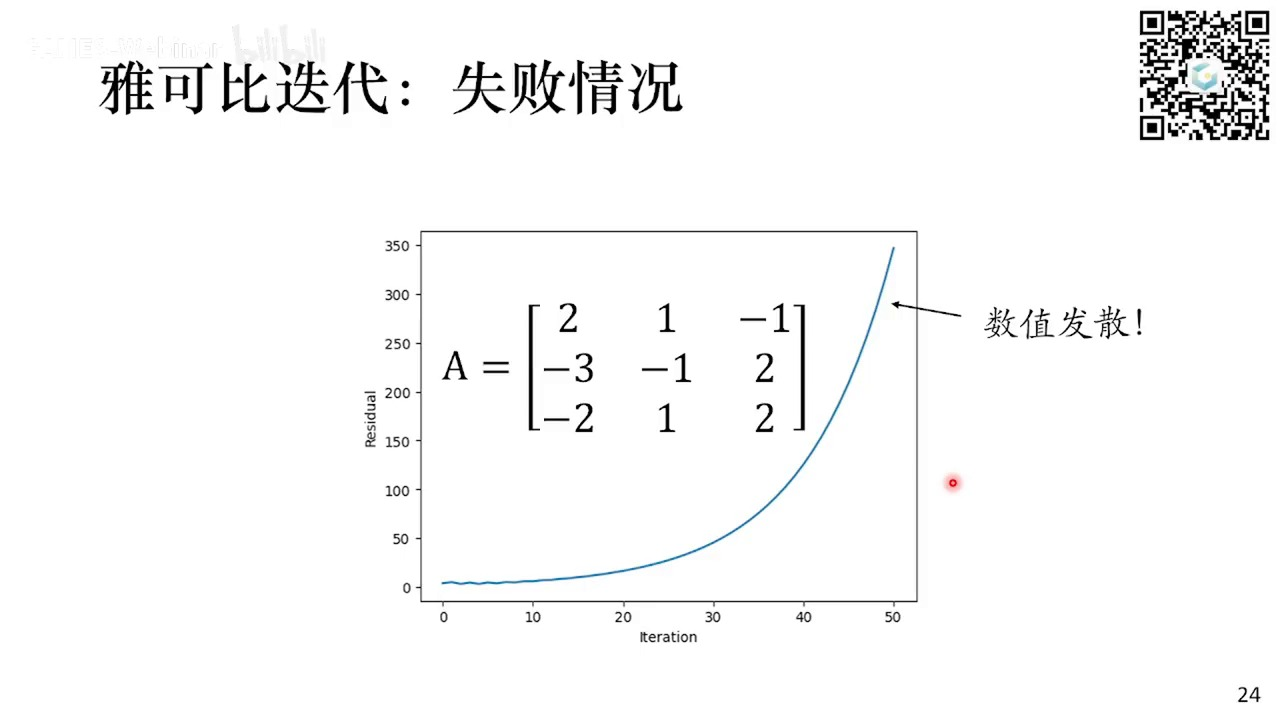
\includegraphics[width=0.92\textwidth]{figures/fig_19_jacobi_fail.jpg}
\caption{雅可比迭代的失败情况：数值发散\vtag}
\end{figure}
\srcnote{00:28:15--00:28:30}
\end{minipage}


但对开头高斯消元例子中的矩阵 $\begin{pmatrix}2&1&-1\\-3&-1&2\\-2&1&2\end{pmatrix}$，残差会一直变大，不会到某个地方就降下来。讲者说，对于这样的矩阵，雅可比迭代失败了，永远不可能达到矩阵的真实解。

\section{不动点迭代的收敛性}

\subsection{误差的传播}

\noindent\begin{minipage}{\textwidth}
\begin{figure}[H]
\centering
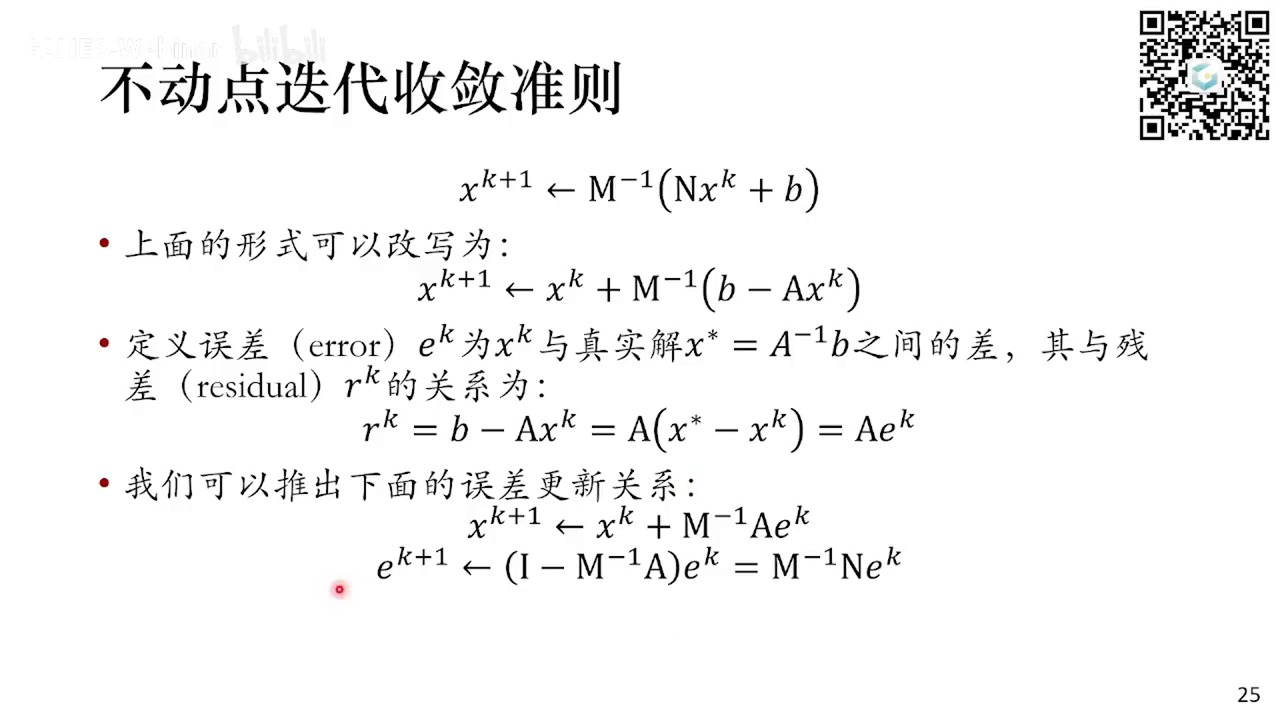
\includegraphics[width=0.92\textwidth]{figures/fig_20_convergence.jpg}
\caption{不动点迭代收敛准则：误差每步乘以迭代矩阵 T\vtag}
\end{figure}
\srcnote{00:30:45--00:31:00}
\end{minipage}


把迭代改写为 $x^{k+1}\leftarrow x^k+\mathrm{M}^{-1}(b-\mathrm{A}x^k)$。定义误差 $e^k$ 为 $x^k$ 与真实解 $x^*=\mathrm{A}^{-1}b$ 之间的差，它与残差 $r^k$ 的关系为
\begin{equation}
r^k=b-\mathrm{A}x^k=\mathrm{A}(x^*-x^k)=\mathrm{A}e^k .
\end{equation}
于是 $x^{k+1}\leftarrow x^k+\mathrm{M}^{-1}\mathrm{A}e^k$，进而得到误差更新关系
\begin{equation}
e^{k+1}\leftarrow(\mathrm{I}-\mathrm{M}^{-1}\mathrm{A})e^k=\mathrm{M}^{-1}\mathrm{N}e^k .
\end{equation}

\subsection{谱半径准则}

在迭代的每一步，误差前面乘上了一个矩阵，称为迭代矩阵 $\mathrm{T}=\mathrm{I}-\mathrm{M}^{-1}\mathrm{A}=\mathrm{M}^{-1}\mathrm{N}$。对 T 做特征值分解 $\mathrm{T}=\mathrm{Q}\Lambda\mathrm{Q}^{-1}$，误差在 Q 的每个特征向量方向上的分量，每迭代一次就乘以对应的特征值。所以：
\begin{itemize}
\item 只有当 T 的所有特征值（包括复数特征值）的模长都小于一时，也即谱半径小于一，反复迭代才能保证 $e^k$ 最终收敛到零；
\item 一旦 T 的特征值中有模长大于一的值，就可能导致不收敛。讲者举例：若 T 是对角矩阵且有一个对角元为 $2$，误差在那一维上每次乘以二，二、四、八、十六，一直变大；
\item 对于 T 特征值越小的分量，误差收敛得越快。
\end{itemize}
极端情况是取 $\mathrm{M}=\mathrm{A}$，此时 $\mathrm{T}=\mathrm{I}-\mathrm{A}^{-1}\mathrm{A}=0$，零矩阵的特征值都是零，一步就能收敛，这是最优的情况。因此应该让 M 尽可能近似 A，同时 $\mathrm{M}^{-1}$ 又可以方便地求解。

\begin{knowledgebox}{一个统一的视角}
所有不动点迭代都在两件事之间权衡：M 越接近 A，迭代矩阵 T 的谱半径越小，收敛所需步数越少；但 M 越接近 A，求 $\mathrm{M}^{-1}$ 作用在向量上也越贵。雅可比取 $\mathrm{M}=\mathrm{D}$，每步最便宜；高斯—赛德尔取下三角部分，每步贵一点但步数更少；取 $\mathrm{M}=\mathrm{A}$ 就退化成直接求解。
\end{knowledgebox}

\subsection{对角占优：一个简单的充分条件}

\noindent\begin{minipage}{\textwidth}
\begin{figure}[H]
\centering
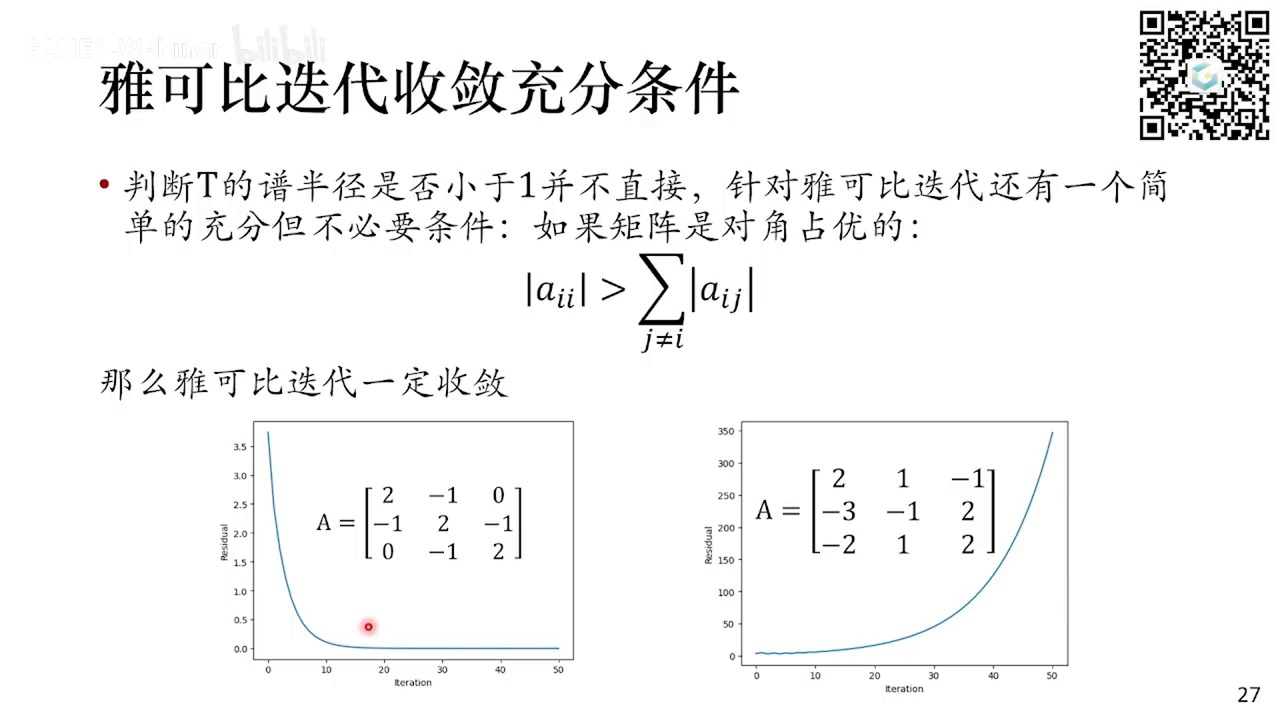
\includegraphics[width=0.92\textwidth]{figures/fig_21_diag_dominant.jpg}
\caption{雅可比迭代收敛的充分条件：对角占优\vtag}
\end{figure}
\srcnote{00:36:45--00:37:00}
\end{minipage}


判断 T 的谱半径是否小于一并不直接，实际应用中不可能把 T 求出来再做特征值分解。针对雅可比迭代有一个简单的充分但不必要条件：如果矩阵是（严格）对角占优的，即每一行对角元的绝对值大于该行所有非对角元素绝对值之和，
\begin{equation}
|a_{ii}|>\sum_{j\ne i}|a_{ij}|,
\end{equation}
那么雅可比迭代一定收敛。

\subsection{松弛}

\noindent\begin{minipage}{\textwidth}
\begin{figure}[H]
\centering
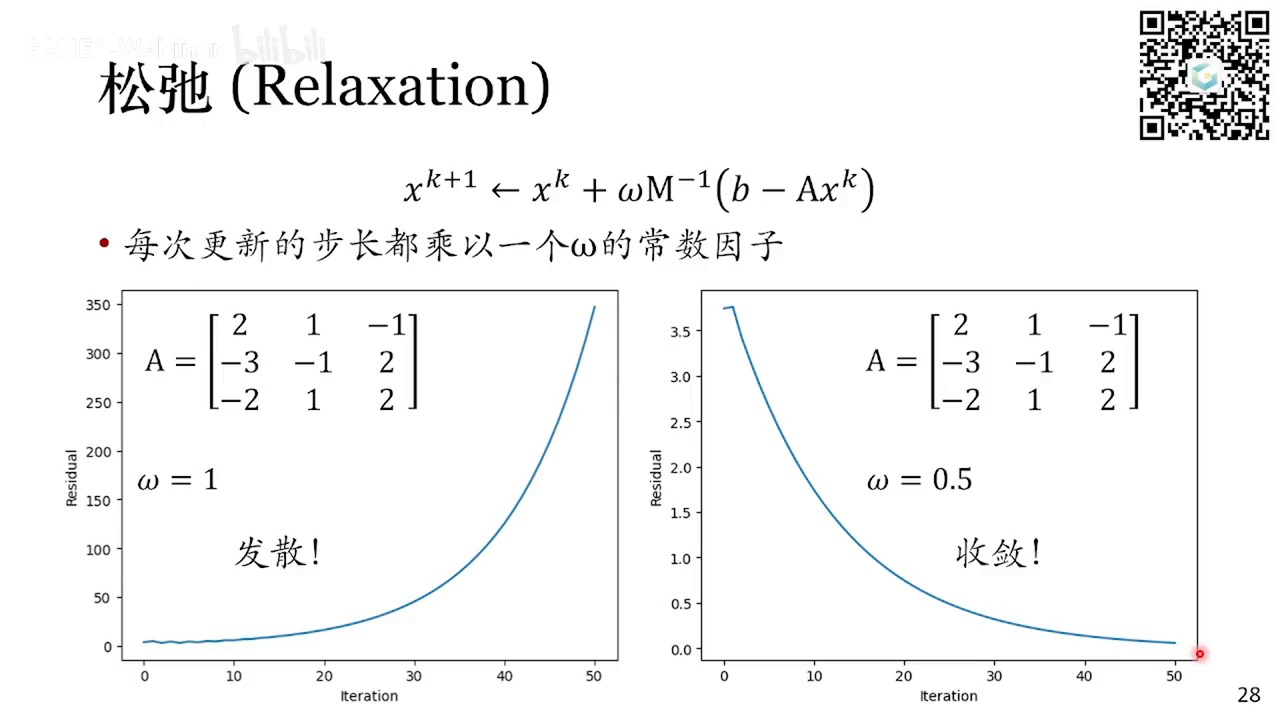
\includegraphics[width=0.92\textwidth]{figures/fig_22_relaxation.jpg}
\caption{松弛：步长乘以常数因子 $\omega$ 后，原本发散的迭代变得收敛\vtag}
\end{figure}
\srcnote{00:38:45--00:39:00}
\end{minipage}


对非对角占优的矩阵，也不是完全没有办法用雅可比迭代去解，可以使用松弛的方法：每次更新的步长都乘以一个常数因子 $\omega$，
\begin{equation}
x^{k+1}\leftarrow x^k+\omega\mathrm{M}^{-1}(b-\mathrm{A}x^k).
\end{equation}
对前面失败的那个矩阵，$\omega=1$ 时发散；取 $\omega=0.5$，即每次更新只走一半的步长，结果最后会收敛，只不过迭代次数相比原来可能多一些。

\begin{practicebox}{为什么松弛能救回发散}
讲义作者补充，读者可以自己推导：加入松弛后，迭代矩阵变为 $\mathrm{T}_\omega=\mathrm{I}-\omega\mathrm{M}^{-1}\mathrm{A}$，它的特征值是 $1-\omega\mu$，其中 $\mu$ 是 $\mathrm{M}^{-1}\mathrm{A}$ 的特征值。若 $\mu$ 都有正实部但有的很大，$\omega=1$ 时 $|1-\mu|$ 可能大于一；适当减小 $\omega$ 就能把所有 $|1-\omega\mu|$ 拉回一以内。代价是收敛变慢，这正是讲者说的“平衡稳定性和收敛速度”。
\end{practicebox}

\subsection{雅可比迭代的速度}

\noindent\begin{minipage}{\textwidth}
\begin{figure}[H]
\centering
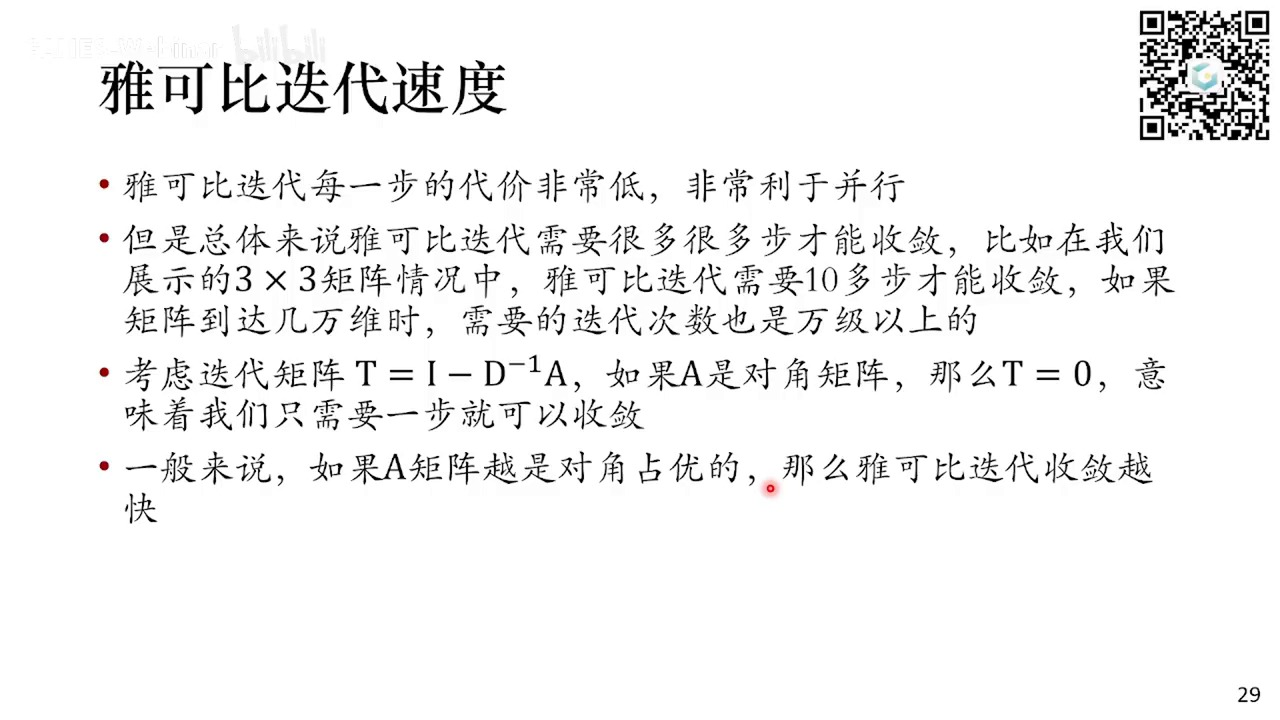
\includegraphics[width=0.92\textwidth]{figures/fig_23_jacobi_speed.jpg}
\caption{雅可比迭代的速度与对角占优程度的关系\vtag}
\end{figure}
\srcnote{00:40:30--00:40:45}
\end{minipage}


雅可比迭代每一步的代价非常低，只需要计算对角矩阵的逆，并且非常利于并行。但总体来说需要很多很多步才能收敛：在展示的 $3\times 3$ 矩阵中，雅可比迭代需要十多步才能收敛；如果矩阵达到几万维，需要的迭代次数也是万级以上。

考虑迭代矩阵 $\mathrm{T}=\mathrm{I}-\mathrm{D}^{-1}\mathrm{A}$：如果 A 是对角矩阵，那么 $\mathrm{T}=0$，一步就可以收敛。反过来说，A 矩阵越是对角占优，对角元越大，雅可比迭代收敛越快。

\section{高斯—赛德尔迭代}

\noindent\begin{minipage}{\textwidth}
\begin{figure}[H]
\centering
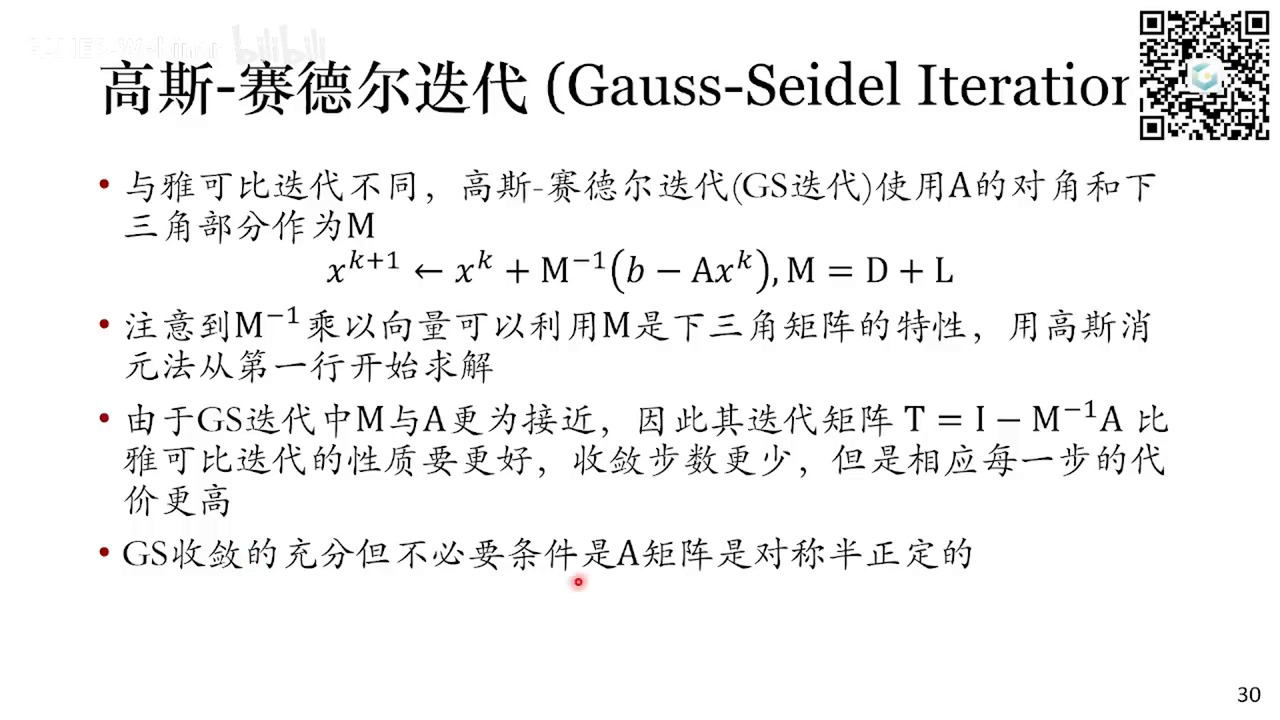
\includegraphics[width=0.92\textwidth]{figures/fig_24_gauss_seidel.jpg}
\caption{高斯—赛德尔迭代：取 A 的对角与下三角部分作为 M\vtag}
\end{figure}
\srcnote{00:43:45--00:44:00}
\end{minipage}


与雅可比迭代不同，高斯—赛德尔迭代（GS 迭代）使用 A 的对角和下三角部分作为 M：
\begin{equation}
x^{k+1}\leftarrow x^k+\mathrm{M}^{-1}(b-\mathrm{A}x^k),\qquad \mathrm{M}=\mathrm{D}+\mathrm{L}.
\end{equation}
M 是下三角矩阵，$\mathrm{M}^{-1}$ 乘以向量就可以利用这一特性，用高斯消元法从第一行开始依次求解，很好算。由于 M 与 A 更为接近，迭代矩阵 $\mathrm{T}=\mathrm{I}-\mathrm{M}^{-1}\mathrm{A}$ 比雅可比迭代的性质更好，收敛步数更少，但相应每一步的代价更高。课件给出 GS 收敛的充分但不必要条件是 A 矩阵对称半正定。

\begin{warningbox}{GS 收敛条件的准确表述}
讲义作者提醒：严格地说，高斯—赛德尔迭代对任意初值都收敛的一个充分条件是 A 对称正定（或严格对角占优）。若 A 只是半正定且奇异，方程可能无解或有无穷多解，迭代不一定收敛到某个确定的解。
\end{warningbox}

\noindent\begin{minipage}{\textwidth}
\begin{figure}[H]
\centering
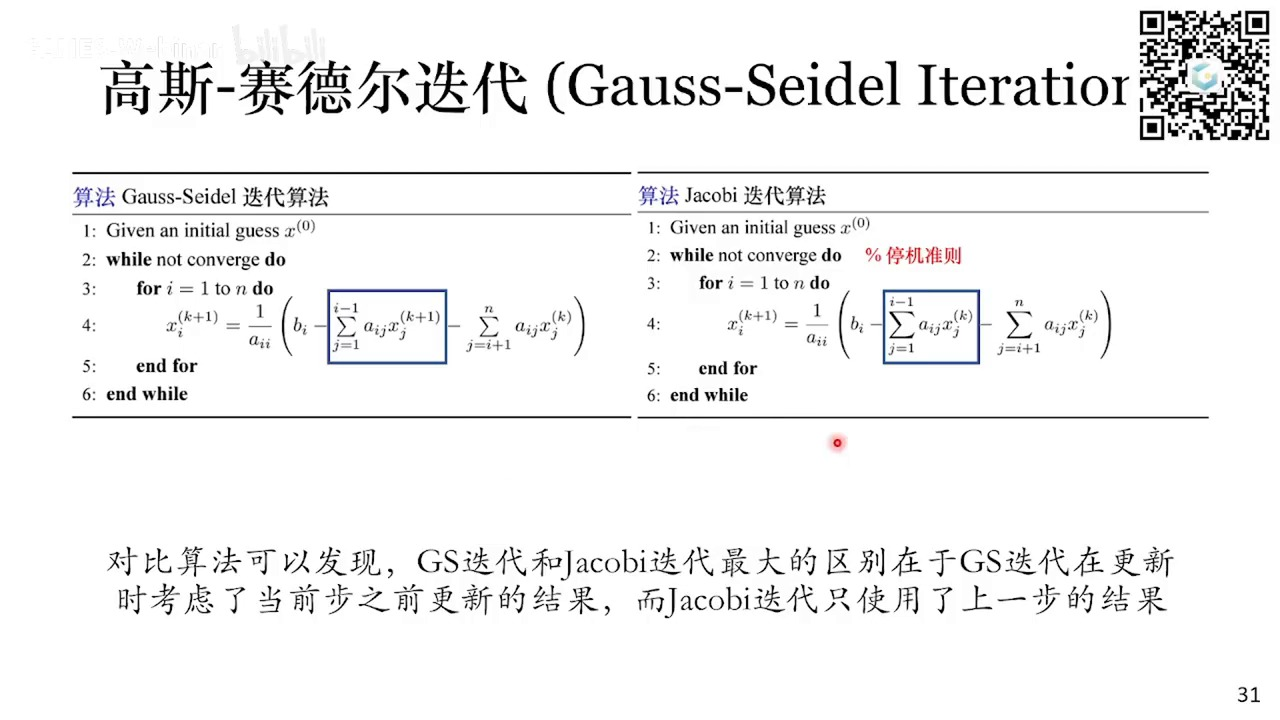
\includegraphics[width=0.92\textwidth]{figures/fig_25_gs_vs_jacobi.jpg}
\caption{对比雅可比迭代与高斯—赛德尔迭代的算法\vtag}
\end{figure}
\srcnote{00:45:00--00:45:15}
\end{minipage}


把两个算法写出来对比，会发现改动非常小：GS 迭代在更新时考虑了当前步之前已经更新的结果，而雅可比迭代只使用上一步的结果。这是两个算法唯一的区别，正是这个区别导致了两者收敛性质的不同，一般来说 GS 迭代比雅可比迭代更快。讲者补充，GS 迭代因为依赖刚更新的值，天然是串行的；但对某些矩阵，可以用重排（例如红黑着色）的方式得到并行版本，感兴趣可以去查一查。

\subsection{不动点迭代总结}

\noindent\begin{minipage}{\textwidth}
\begin{figure}[H]
\centering
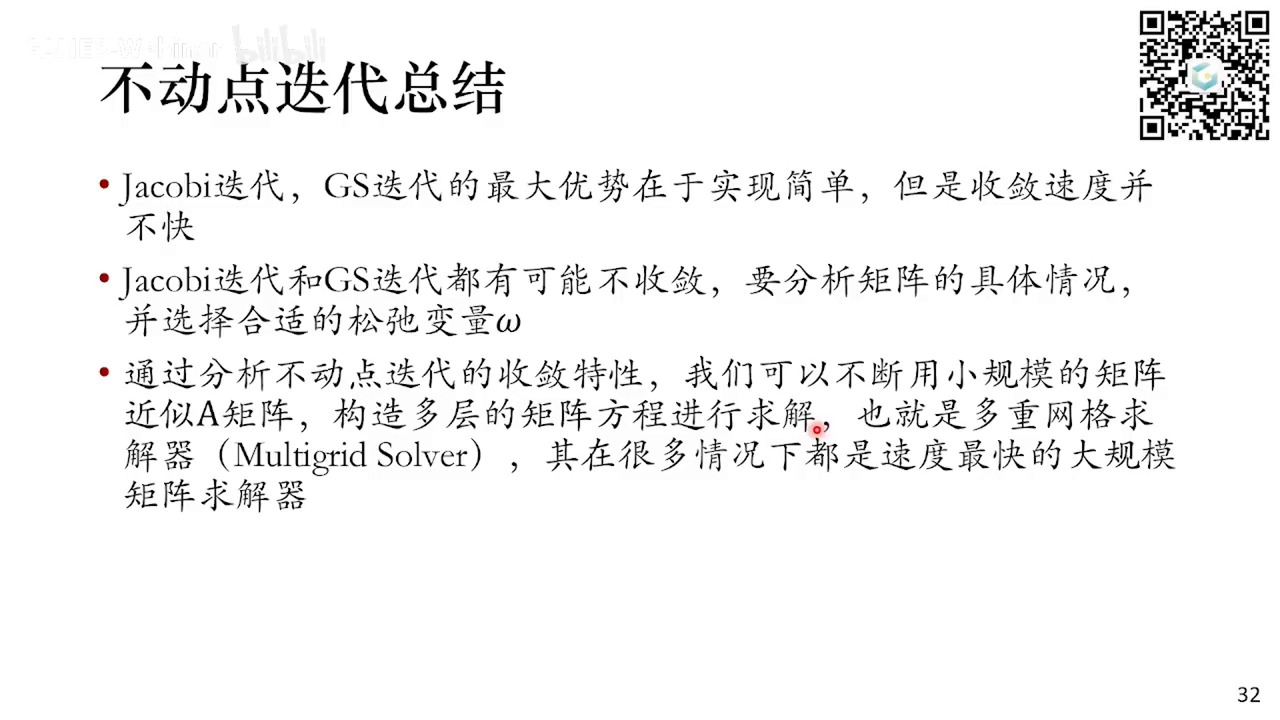
\includegraphics[width=0.92\textwidth]{figures/fig_26_stationary_summary.jpg}
\caption{不动点迭代总结与多重网格的思想\vtag}
\end{figure}
\srcnote{00:47:45--00:48:00}
\end{minipage}


雅可比迭代和 GS 迭代的最大优势在于实现简单，但收敛速度并不快。两者都有可能不收敛，要具体分析矩阵的情况，并选择合适的松弛变量 $\omega$。通过分析不动点迭代的收敛特性，还可以不断用小规模的矩阵近似 A，构造多层的矩阵方程进行求解，在不同层上做不动点迭代，这就是多重网格求解器（multigrid solver）的基本思想，它在很多情况下是速度最快的大规模矩阵求解器。讲者说多重网格今天不展开，感兴趣可以自行了解。

\section{第二类：子空间迭代}

\subsection{基本思想}

\noindent\begin{minipage}{\textwidth}
\begin{figure}[H]
\centering
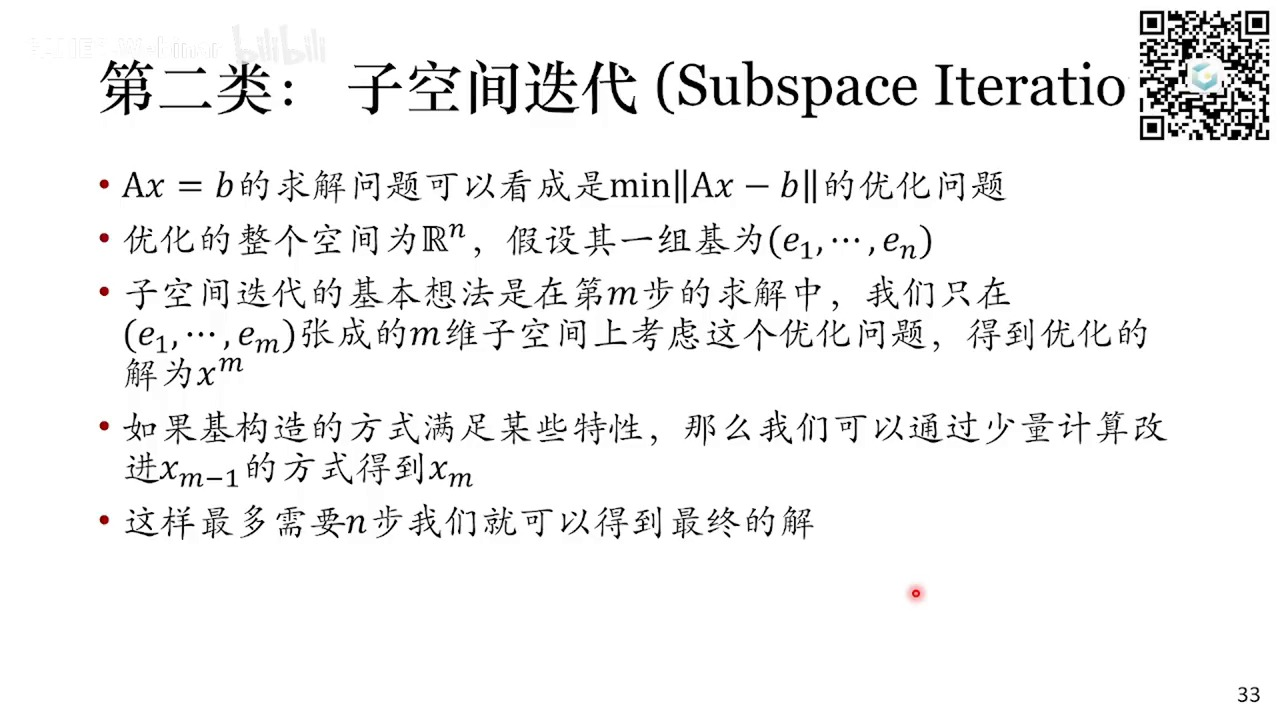
\includegraphics[width=0.92\textwidth]{figures/fig_27_subspace.jpg}
\caption{子空间迭代的基本想法\vtag}
\end{figure}
\srcnote{00:51:45--00:52:00}
\end{minipage}


到目前为止介绍了直接求解方法（LU 分解和 $\mathrm{LL}^{\mathsf T}$ 分解）和不动点迭代方法（雅可比迭代和 GS 迭代）。第三种是子空间迭代。$\mathrm{A}x=b$ 的求解问题可以看成 $\min\|\mathrm{A}x-b\|$ 的优化问题，整个优化空间为 $\mathbb R^n$，假设其一组基为 $(e_1,\dots,e_n)$。子空间迭代的基本想法是：在第 $m$ 步的求解中，只在 $(e_1,\dots,e_m)$ 张成的 $m$ 维子空间上考虑这个优化问题，得到优化的解为 $x_m$。如果基构造的方式满足某些特性，就可以通过少量计算改进 $x_{m-1}$ 得到 $x_m$。这样最多需要 $n$ 步就可以得到最终的解，因为第 $n$ 步时子空间就是全空间。

\subsection{Krylov 子空间}

\noindent\begin{minipage}{\textwidth}
\begin{figure}[H]
\centering
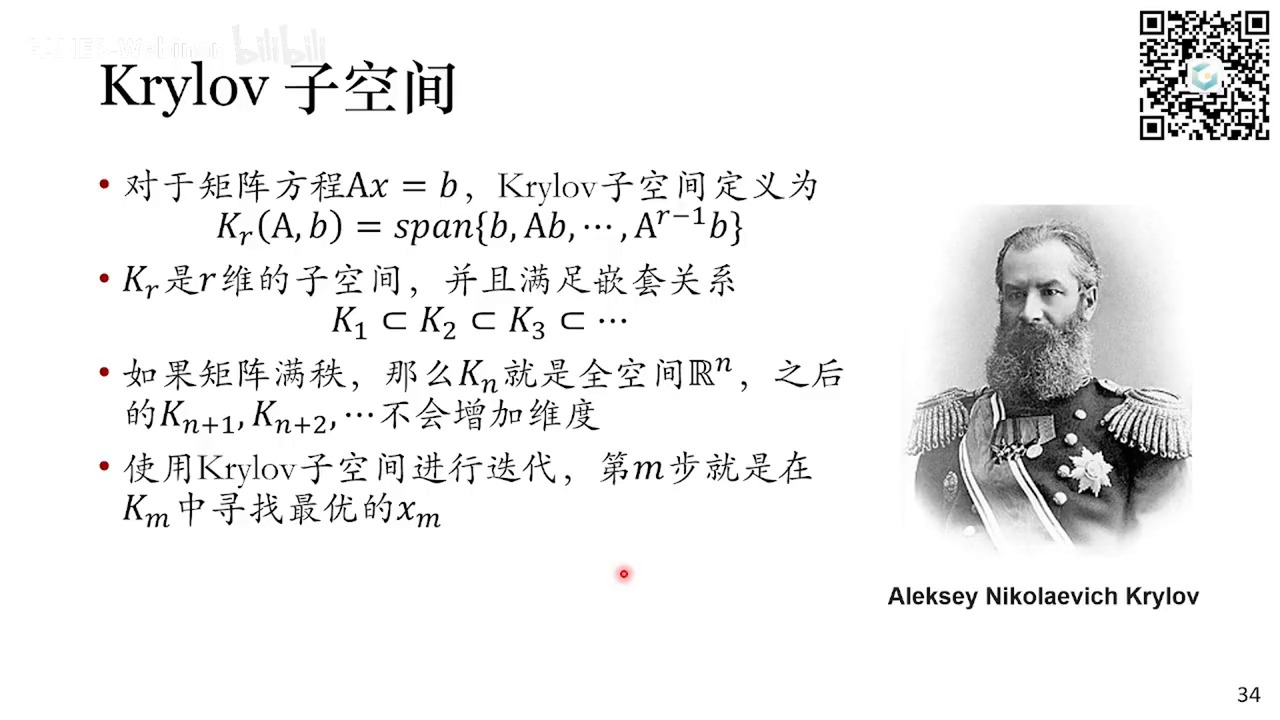
\includegraphics[width=0.92\textwidth]{figures/fig_28_krylov.jpg}
\caption{Krylov 子空间的定义与嵌套关系\vtag}
\end{figure}
\srcnote{00:54:45--00:55:00}
\end{minipage}


最成功的子空间方法是基于 Krylov 子空间的方法，Krylov 是俄国数学家。对于矩阵方程 $\mathrm{A}x=b$，Krylov 子空间定义为
\begin{equation}
K_r(\mathrm{A},b)=\operatorname{span}\{b,\mathrm{A}b,\dots,\mathrm{A}^{r-1}b\}.
\end{equation}
$K_r$ 是 $r$ 维的子空间，并且满足嵌套关系 $K_1\subset K_2\subset K_3\subset\cdots$。如果矩阵满秩，那么 $K_n$ 就是全空间 $\mathbb R^n$，之后的 $K_{n+1},K_{n+2},\dots$ 虽然向量个数变多，但空间维度不再增加。使用 Krylov 子空间进行迭代，第 $m$ 步就是在 $K_m$ 中寻找最优的 $x_m$。

\section{共轭梯度下降}

\subsection{问题的转化}

\noindent\begin{minipage}{\textwidth}
\begin{figure}[H]
\centering
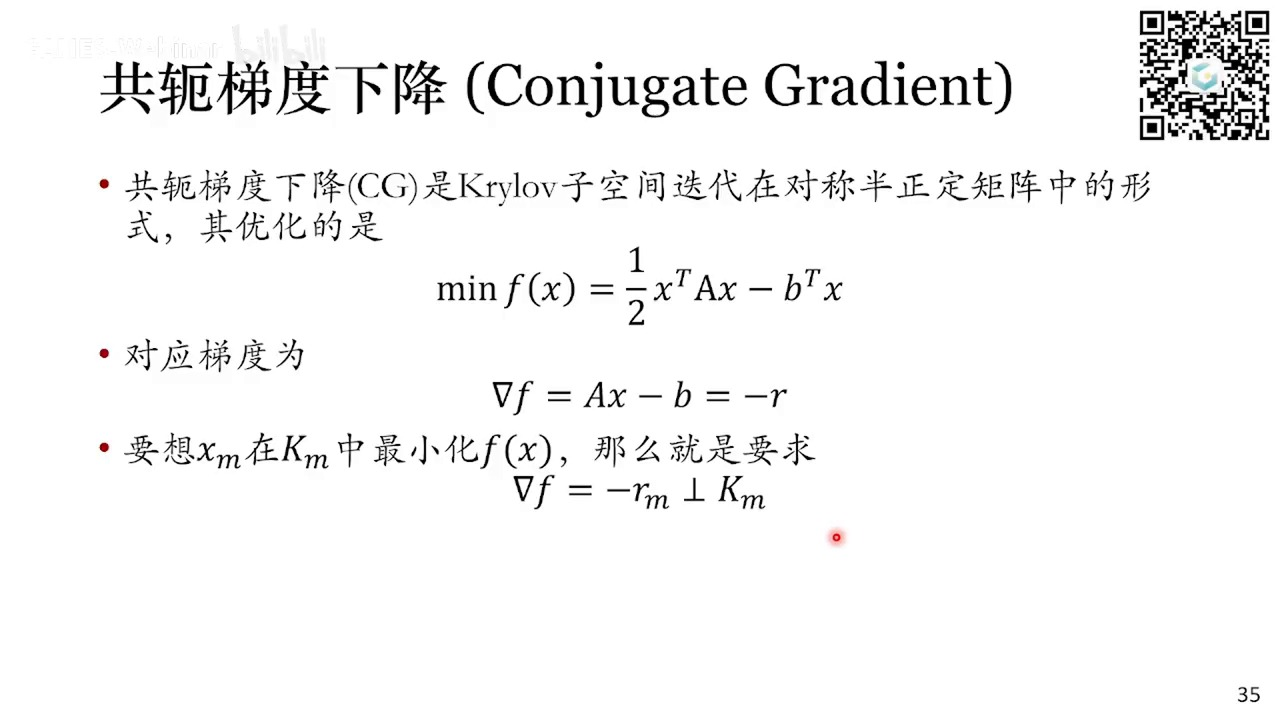
\includegraphics[width=0.92\textwidth]{figures/fig_29_cg_objective.jpg}
\caption{共轭梯度下降：对称正定矩阵上的二次优化\vtag}
\end{figure}
\srcnote{00:58:00--00:58:15}
\end{minipage}


共轭梯度下降（conjugate gradient，CG）是 Krylov 子空间迭代在对称正定矩阵上的形式，它把 $\mathrm{A}x=b$ 转化为
\begin{equation}
\min f(x)=\frac{1}{2}x^{\mathsf T}\mathrm{A}x-b^{\mathsf T}x ,
\end{equation}
对应梯度为 $\nabla f=\mathrm{A}x-b=-r$。梯度为零时就有 $\mathrm{A}x=b$，所以求最小值等价于解方程。要想 $x_m$ 在 $K_m$ 中最小化 $f(x)$，就要求 $\nabla f=-r_m\perp K_m$。讲者解释这个几何结论：如果梯度与子空间正交，就意味着在子空间中沿任何方向移动都无法再进一步减小 $f$ 的值。

\subsection{共轭基}

\noindent\begin{minipage}{\textwidth}
\begin{figure}[H]
\centering
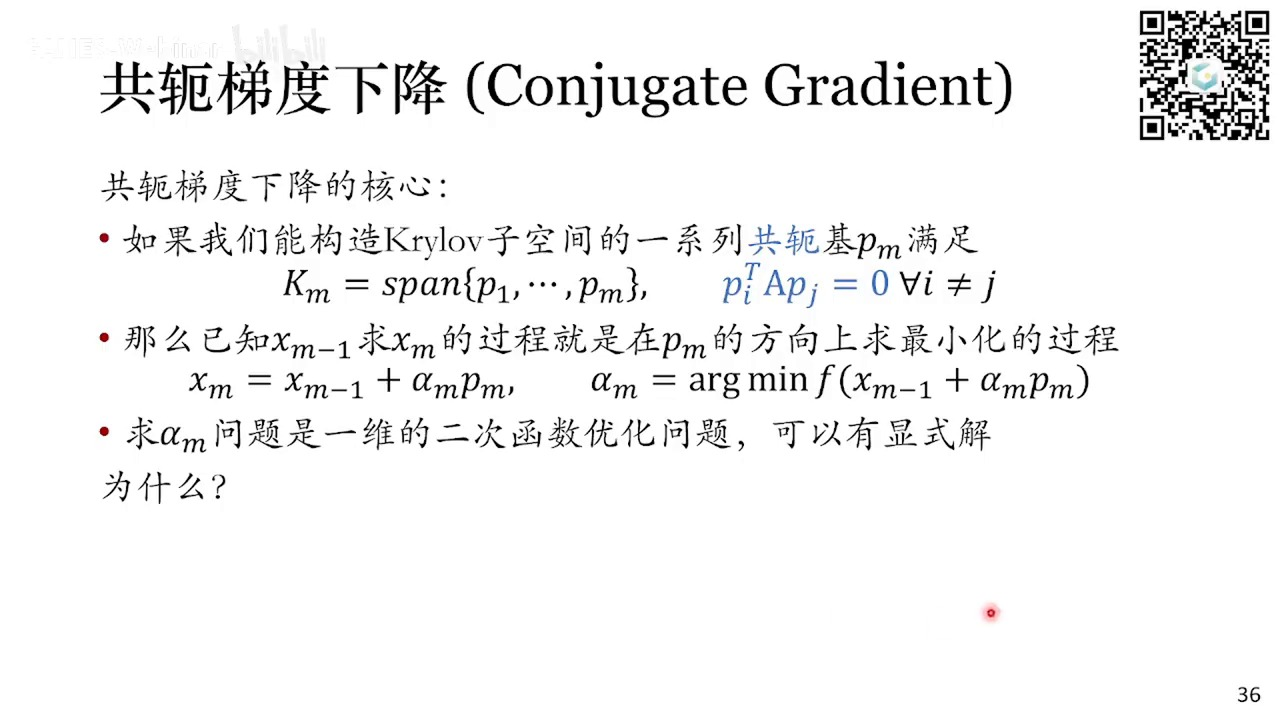
\includegraphics[width=0.92\textwidth]{figures/fig_30_cg_core.jpg}
\caption{共轭梯度下降的核心：构造 Krylov 子空间的共轭基\vtag}
\end{figure}
\srcnote{01:01:15--01:01:30}
\end{minipage}


共轭梯度下降的核心是：如果能构造 Krylov 子空间的一系列共轭基 $p_m$，满足
\begin{equation}
K_m=\operatorname{span}\{p_1,\dots,p_m\},\qquad p_i^{\mathsf T}\mathrm{A}p_j=0\quad\forall i\ne j,
\end{equation}
那么已知 $x_{m-1}$ 求 $x_m$ 的过程，就是在 $p_m$ 方向上求最小化的过程：
\begin{equation}
x_m=x_{m-1}+\alpha_mp_m,\qquad \alpha_m=\arg\min_{\alpha} f(x_{m-1}+\alpha p_m).
\end{equation}
$\alpha_m$ 是标量，$p_m$ 是已知方向，所以这是一维的二次函数优化问题，有显式解。课件在这里问“为什么”，讲义作者补充答案：把 $f(x_{m-1}+\alpha p_m)$ 展开是 $\alpha$ 的二次函数，求导令其为零即得 $\alpha_m=\frac{p_m^{\mathsf T}r_{m-1}}{p_m^{\mathsf T}\mathrm{A}p_m}$。

\subsection{归纳证明}

\noindent\begin{minipage}{\textwidth}
\begin{figure}[H]
\centering
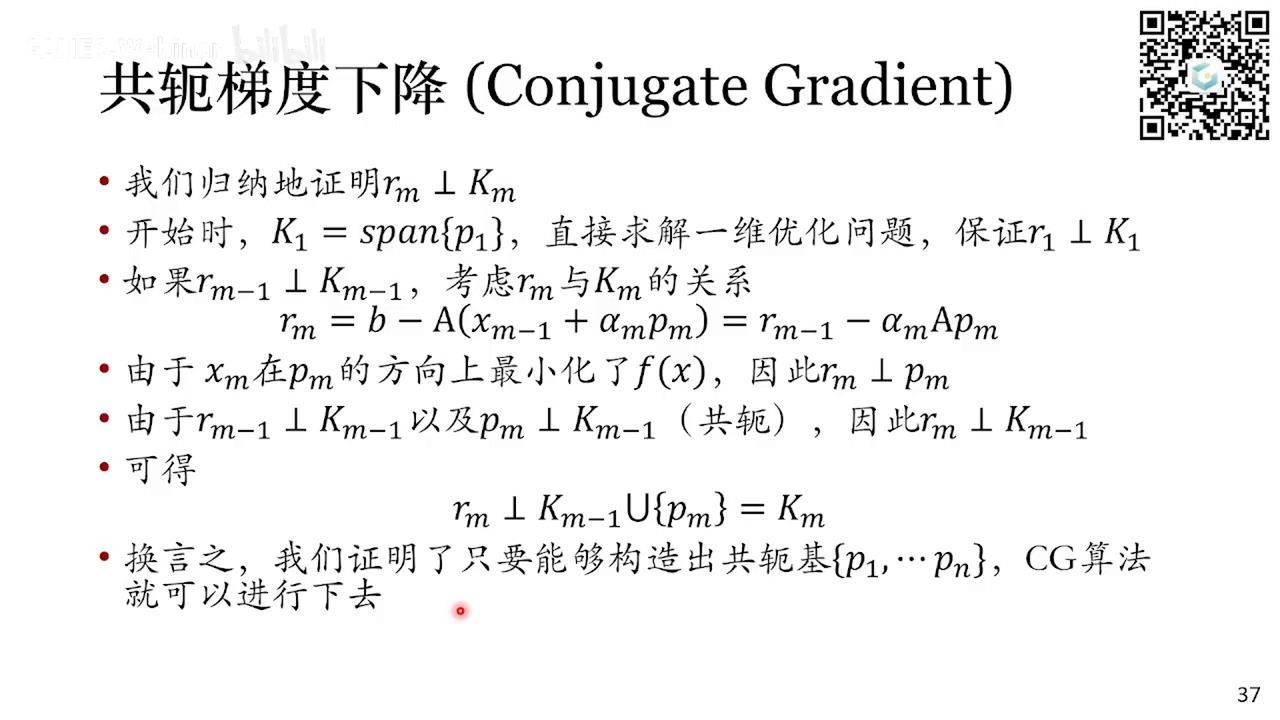
\includegraphics[width=0.92\textwidth]{figures/fig_31_cg_proof.jpg}
\caption{归纳证明 $r_m\perp K_m$\vtag}
\end{figure}
\srcnote{01:05:45--01:06:00}
\end{minipage}


讲者归纳地证明 $r_m\perp K_m$。开始时 $K_1=\operatorname{span}\{p_1\}$，直接求解一维优化问题，保证 $r_1\perp K_1$。若 $r_{m-1}\perp K_{m-1}$，考虑 $r_m$ 与 $K_m$ 的关系：
\begin{equation}
r_m=b-\mathrm{A}(x_{m-1}+\alpha_mp_m)=r_{m-1}-\alpha_m\mathrm{A}p_m .
\end{equation}
由于 $x_m$ 在 $p_m$ 方向上最小化了 $f(x)$，因此 $r_m\perp p_m$；由于 $r_{m-1}\perp K_{m-1}$，以及构造基时用到的共轭关系使 $\mathrm{A}p_m\perp K_{m-1}$，因此 $r_m\perp K_{m-1}$。可得 $r_m\perp K_{m-1}\cup\{p_m\}$，即 $r_m\perp K_m$。换言之，只要能构造出共轭基 $\{p_1,\dots,p_n\}$，CG 算法就可以进行下去。

\subsection{算法}

\noindent\begin{minipage}{\textwidth}
\begin{figure}[H]
\centering
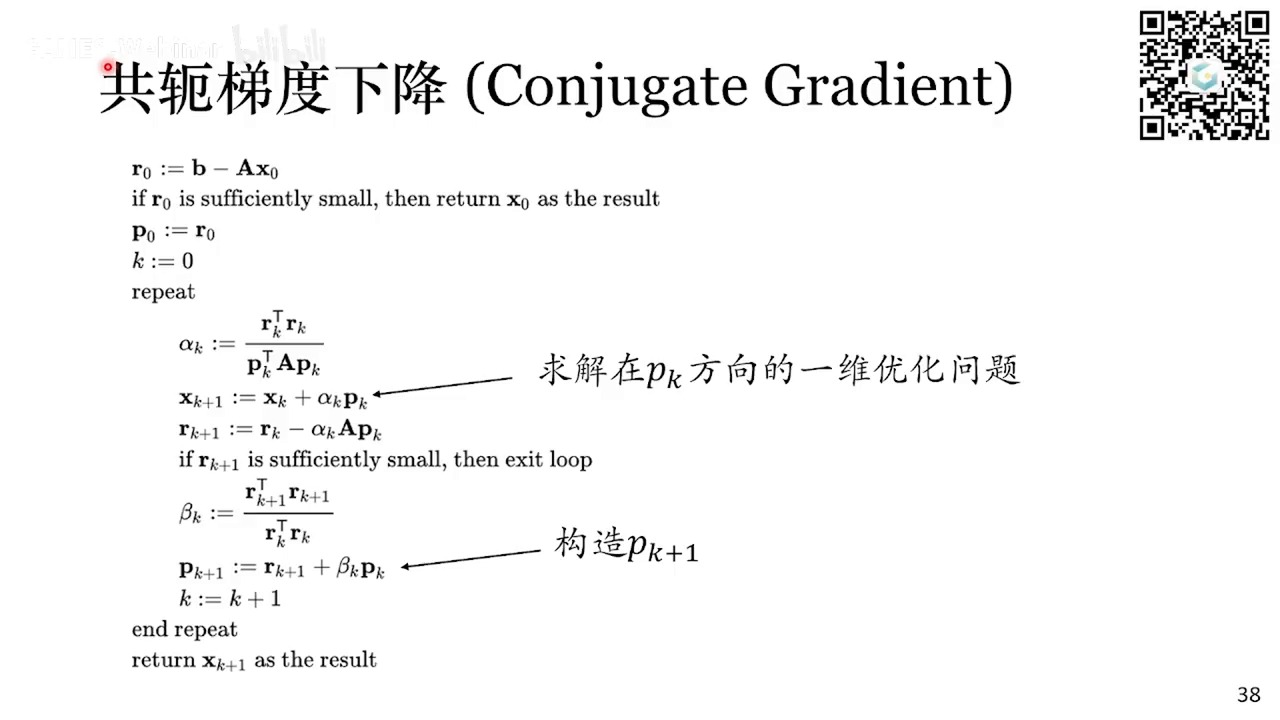
\includegraphics[width=0.92\textwidth]{figures/fig_32_cg_algo.jpg}
\caption{共轭梯度下降算法：一维优化求步长，再构造下一个共轭方向\vtag}
\end{figure}
\srcnote{01:07:45--01:08:00}
\end{minipage}


讲者没有展开构造共轭基的推导，直接给出算法的具体形式。前一部分求 $\alpha_k$，就是在 $p_k$ 方向上解一维优化问题；后一部分构造 $p_{k+1}=r_{k+1}+\beta_kp_k$，也是一步更新，新方向只需要由当前残差和上一个方向组合得到。这依赖 Krylov 子空间的一些独特性质，今天不细讲。写成完整的迭代为
\begin{equation}
\begin{gathered}
\alpha_k=\frac{r_k^{\mathsf T}r_k}{p_k^{\mathsf T}\mathrm{A}p_k},\qquad x_{k+1}=x_k+\alpha_kp_k,\qquad r_{k+1}=r_k-\alpha_k\mathrm{A}p_k,\\
\beta_k=\frac{r_{k+1}^{\mathsf T}r_{k+1}}{r_k^{\mathsf T}r_k},\qquad p_{k+1}=r_{k+1}+\beta_kp_k .
\end{gathered}
\end{equation}

\subsection{收敛速度}

\noindent\begin{minipage}{\textwidth}
\begin{figure}[H]
\centering
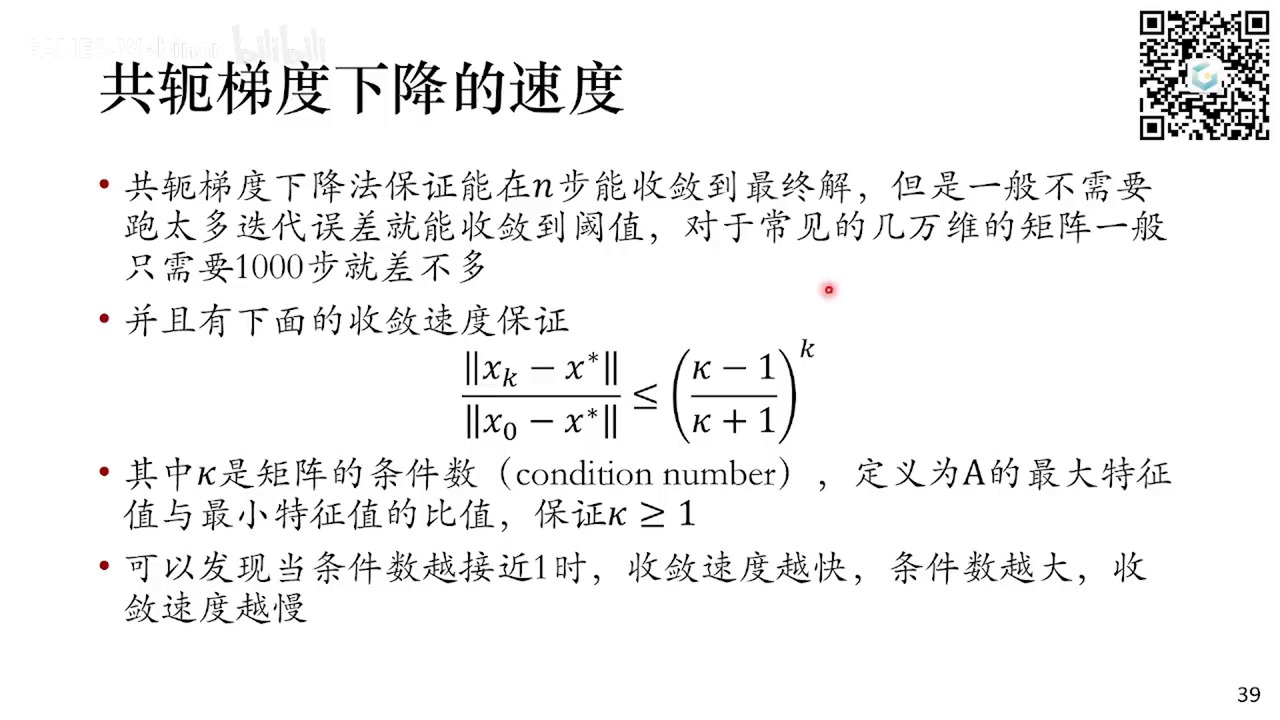
\includegraphics[width=0.92\textwidth]{figures/fig_33_cg_speed.jpg}
\caption{共轭梯度下降的速度与条件数\vtag}
\end{figure}
\srcnote{01:10:30--01:10:45}
\end{minipage}


共轭梯度下降法保证在 $n$ 步内收敛到最终解，但一般不需要跑那么多步，迭代远少于 $n$ 步时误差基本上就能降到阈值以下。讲者说，对于常见的几万维矩阵，一般只需要一千步左右（口头说几千步）就差不多。并且有下面的收敛速度保证：
\begin{equation}
\frac{\|x_k-x^*\|}{\|x_0-x^*\|}\le\left(\frac{\kappa-1}{\kappa+1}\right)^k,
\end{equation}
其中 $\kappa$ 是矩阵的条件数，定义为 A 的最大特征值与最小特征值的比值，保证 $\kappa\ge 1$。条件数越接近一，底数越接近零，收敛越快，相当于每一步误差都乘以零点一、零点零一这样的小数；条件数越大，收敛越慢。

\begin{knowledgebox}{条件数的直观含义}
讲义作者补充：对称正定矩阵的二次函数 $f(x)=\frac12x^{\mathsf T}\mathrm{A}x-b^{\mathsf T}x$ 的等值线是椭球，椭球最长轴与最短轴之比的平方就是条件数。条件数为一时等值线是圆，沿负梯度一步就到中心；条件数很大时椭球被拉得又扁又长，梯度方向几乎不指向中心，迭代只能在峡谷里来回折返。预处理相当于先把椭球“压圆”。
\end{knowledgebox}

\begin{warningbox}{CG 收敛界的常见形式}
讲义作者提醒：教科书中 CG 更常见、也更紧的界是用 A 范数写的
$\|x_k-x^*\|_{\mathrm A}\le 2\left(\frac{\sqrt\kappa-1}{\sqrt\kappa+1}\right)^k\|x_0-x^*\|_{\mathrm A}$，
底数里是 $\sqrt\kappa$；不带根号的 $\frac{\kappa-1}{\kappa+1}$ 是最速下降法的收敛因子。两者传达的结论相同：条件数越小越快，但 CG 对条件数的依赖要温和得多。
\end{warningbox}

\section{预处理与其他 Krylov 求解器}

\subsection{预处理}

\noindent\begin{minipage}{\textwidth}
\begin{figure}[H]
\centering
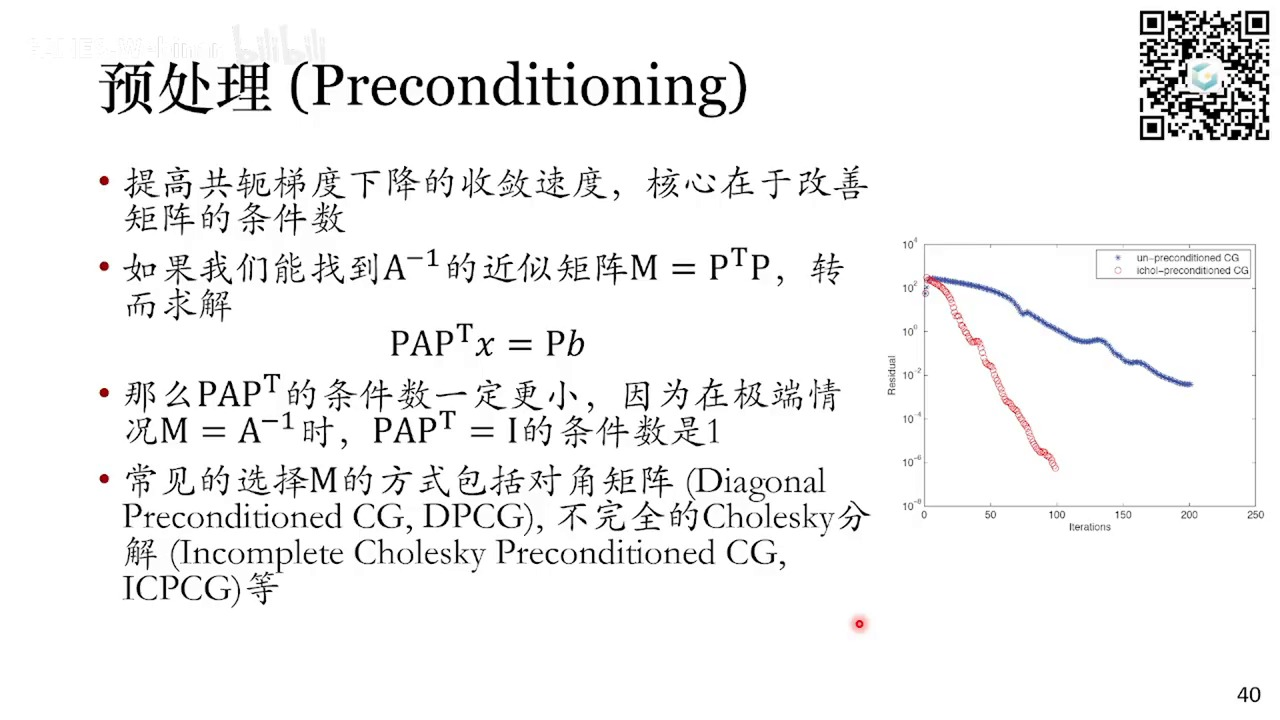
\includegraphics[width=0.92\textwidth]{figures/fig_34_precond.jpg}
\caption{预处理：用 $\mathrm{A}^{-1}$ 的近似改善条件数\vtag}
\end{figure}
\srcnote{01:13:30--01:13:45}
\end{minipage}


提高共轭梯度下降的收敛速度，核心在于改善矩阵的条件数。如果能找到 $\mathrm{A}^{-1}$ 的近似矩阵 $\mathrm{M}=\mathrm{P}^{\mathsf T}\mathrm{P}$，转而求解
\begin{equation}
\mathrm{PAP}^{\mathsf T}y=\mathrm{P}b,\qquad x=\mathrm{P}^{\mathsf T}y ,
\end{equation}
那么 $\mathrm{PAP}^{\mathsf T}$ 的条件数一定更小，因为在极端情况 $\mathrm{M}=\mathrm{A}^{-1}$ 时，$\mathrm{PAP}^{\mathsf T}=\mathrm{I}$，条件数是一。这个方程对 CG 来说就会收敛得非常快。

如何选择 M？与前面不动点迭代有些类似。常见的选择包括：直接把 M 选成 A 的对角部分的逆，称为对角预处理共轭梯度（diagonal preconditioned CG，DPCG）；用最开始介绍的 $\mathrm{LL}^{\mathsf T}$ 分解，但只做不完全的科列斯基分解，称为 ICPCG（incomplete Cholesky preconditioned CG）。讲者说，预处理是非常强大的技术，ICPCG 是求解对称正定矩阵方程时非常常用的求解器，对几万维的矩阵甚至只需要几十步就可以收敛。

\begin{knowledgebox}{不完全科列斯基分解}
讲义作者补充：对稀疏矩阵做完整的科列斯基分解，L 中会出现大量原本为零的位置变成非零（填充），既费内存又费时间。不完全分解只保留 A 原有非零位置上的元素，丢掉填充，得到的 $\mathrm{LL}^{\mathsf T}$ 只是 A 的近似，但计算便宜，作为预处理器效果往往很好。
\end{knowledgebox}

\subsection{其他 Krylov 子空间求解器}

\noindent\begin{minipage}{\textwidth}
\begin{figure}[H]
\centering
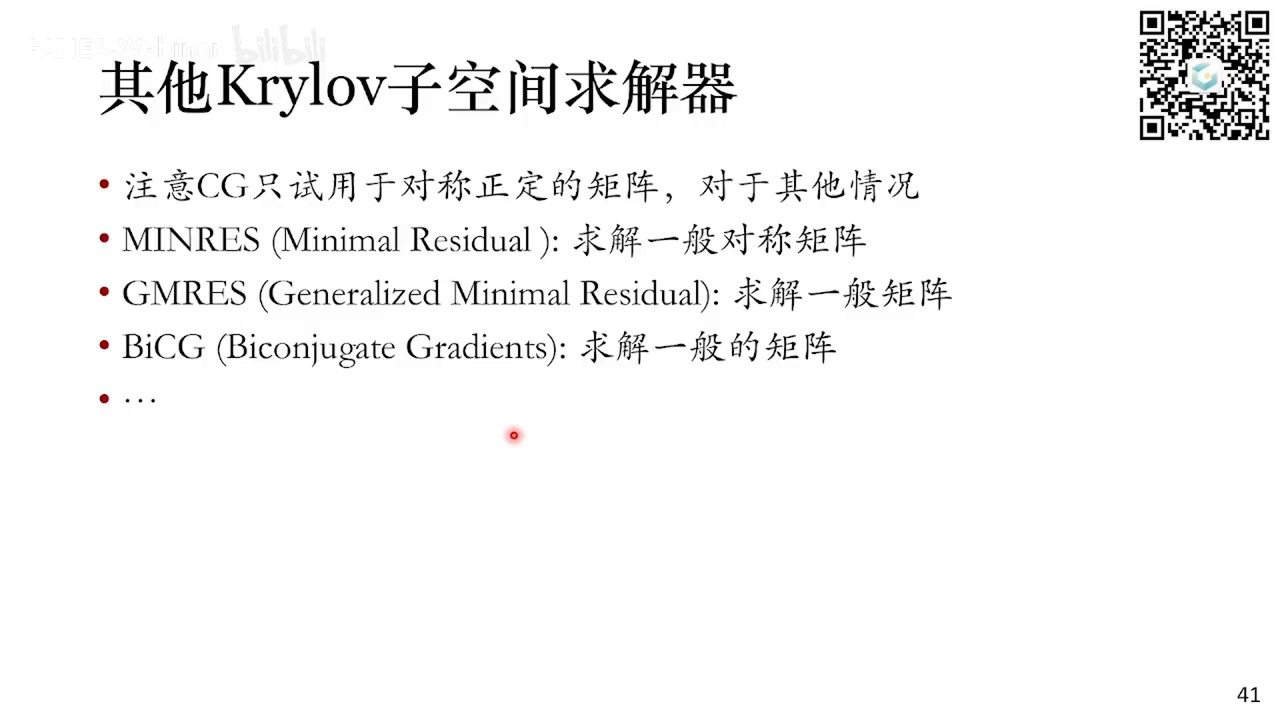
\includegraphics[width=0.92\textwidth]{figures/fig_35_other_krylov.jpg}
\caption{其他 Krylov 子空间求解器\vtag}
\end{figure}
\srcnote{01:15:00--01:15:15}
\end{minipage}


注意 CG 只适用于对称正定的矩阵。对于其他情况，也有相应的 Krylov 子空间求解器：
\begin{itemize}
\item MINRES（minimal residual）：求解一般的对称矩阵，不一定正定；
\item GMRES（generalized minimal residual）：求解一般矩阵；
\item BiCG（biconjugate gradients）以及 BiCGSTAB：求解一般的矩阵。
\end{itemize}

\section{总结}

\noindent\begin{minipage}{\textwidth}
\begin{figure}[H]
\centering
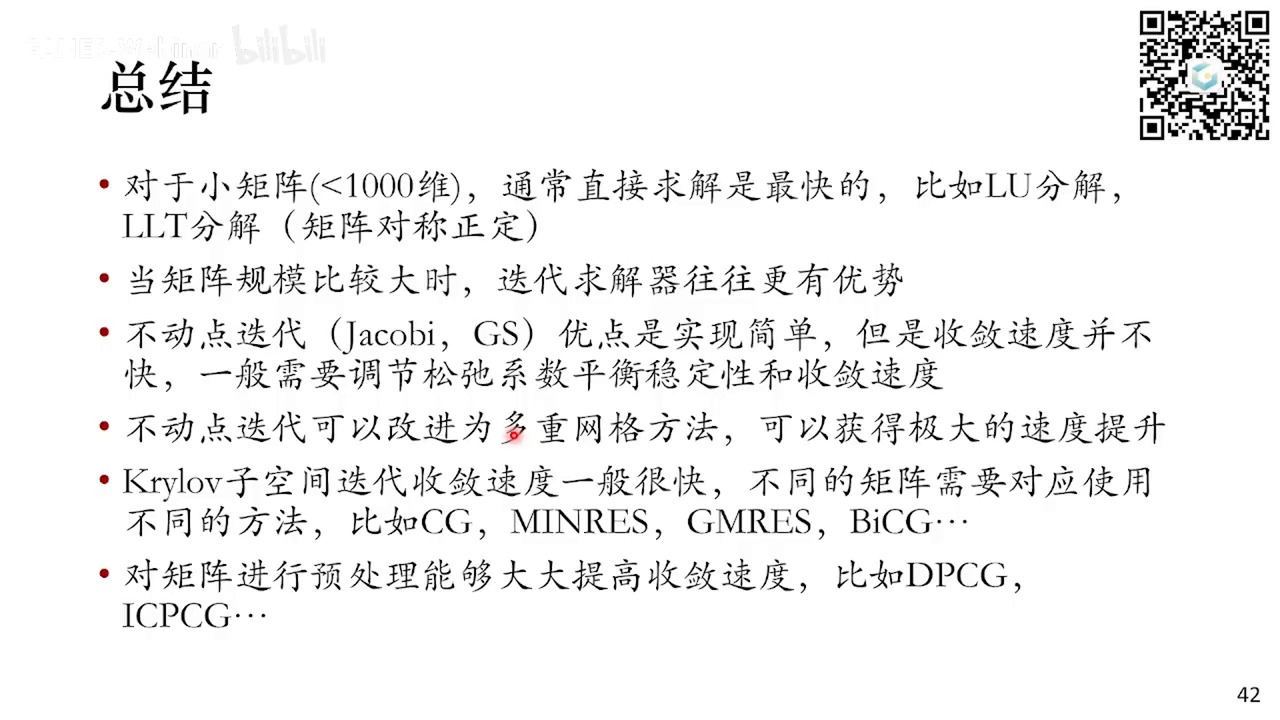
\includegraphics[width=0.92\textwidth]{figures/fig_36_summary.jpg}
\caption{本讲总结\vtag}
\end{figure}
\srcnote{01:17:45--01:18:00}
\end{minipage}


讲者总结了今天的内容：
\begin{itemize}
\item 对于小矩阵（小于 $1000$ 维），通常直接求解是最快的，比如 LU 分解，或矩阵对称正定时用 $\mathrm{LL}^{\mathsf T}$ 分解；
\item 当矩阵规模比较大时，迭代求解器往往更有优势；
\item 不动点迭代（雅可比、GS）优点是实现简单，但收敛速度并不快，一般需要调节松弛系数平衡稳定性和收敛速度；
\item 不动点迭代可以改进为多重网格方法，获得极大的速度提升；
\item Krylov 子空间迭代收敛速度一般很快，不同的矩阵需要对应使用不同的方法，比如 CG、MINRES、GMRES、BiCG 等；
\item 对矩阵进行预处理能够大大提高收敛速度，比如 DPCG、ICPCG 等。
\end{itemize}
讲者强调，对于 $\mathrm{A}x=b$ 问题，没有通用的最优求解器，还是要根据实际情况选择合适的求解器。今天提到的这些求解器，在 NumPy、SciPy、MATLAB 等数学库里都有实现，可以直接调用。本讲的作业是几个代码填空题，没有理论作业，对应课件里的算法流程把空补上，可以跑一跑，比较不同求解器的表现。

\begin{importantbox}{选择求解器的简单流程}
按讲者的总结，可以整理成一个粗略的决策顺序：矩阵很小，直接分解；矩阵大且对称正定，用带预处理的共轭梯度（DPCG、ICPCG）；对称但不定，用 MINRES；一般非对称矩阵，用 GMRES 或 BiCGSTAB；问题有网格结构、规模极大，考虑多重网格；只需要粗糙解或要求极简实现，雅可比或 GS 迭代加松弛。
\end{importantbox}

\begin{practicebox}{自测}
\begin{enumerate}
\item 对开头的三阶例子，验证 $\mathrm{L}$ 与 $\mathrm{U}$ 的乘积确实等于 A，并用前代和回代解出 $x=(2,3,-1)^{\mathsf T}$。
\item 判断三对角矩阵 $\mathrm{tridiag}(-1,2,-1)$ 是否严格对角占优；它不是严格对角占优，但雅可比迭代仍然收敛，这说明了什么？
\item 写出雅可比迭代和 GS 迭代的迭代矩阵 T，并说明为什么 $\mathrm{M}=\mathrm{A}$ 时一步收敛。
\item 若矩阵条件数 $\kappa=100$，按课件的收敛界，误差降到初始的千分之一大约需要多少步？（提示：$\left(\frac{99}{101}\right)^k\le 10^{-3}$，约 $346$ 步。）
\end{enumerate}
\end{practicebox}

讲者给出的参考资料包括：华东师范大学潘建瑜老师的数值分析课程讲义，MATLAB 的函数文档，《An Introduction to the Conjugate Gradient Method Without the Agonizing Pain》，以及《A Sampler of Useful Computational Tools for Applied Geometry, Computer Graphics, and Image Processing》。

\end{document}
